\documentclass{article}

\usepackage{graphicx}
\usepackage{hyperref}
\usepackage[a4paper, margin=1in]{geometry}
\usepackage{breakcites}
\usepackage{subcaption}
\usepackage{float}
\usepackage{textcomp}
\usepackage{amsmath}
\usepackage{textgreek}
\usepackage{authblk}
\usepackage{rotating}
\usepackage{booktabs}
\usepackage{longtable}
\usepackage{pdflscape}
\usepackage{subcaption}
\usepackage{lineno}
\usepackage{fancyhdr}
\usepackage[
  style=numeric,
  citestyle=numeric-comp,
  backend=biber,
  doi=true,
  natbib=true,
  sorting=none
]{biblatex}
\usepackage{lineno}

\linenumbers


\pagestyle{fancy}
\fancyhf{}
\lfoot{Supplemental Materials for \textit{Neighborhood Income and Race Moderate the Effect of Heat on Expressed Mood}}
\rfoot{\thepage}

\renewcommand{\footrulewidth}{0.4pt}
\renewcommand{\headrulewidth}{0pt}


\addbibresource{TextDataClimateShocks.bib}

\begin{document}
\begin{center}
\section*{Supplemental Materials for \textit{Neighborhood Income and Race Moderate the Effect of Heat on Expressed Mood}}
\end{center}

\setcounter{table}{0}
\setcounter{figure}{0}
\setcounter{section}{0}
\renewcommand{\thetable}{S\arabic{table}}
\renewcommand{\thefigure}{S\arabic{figure}}
\renewcommand{\thesection}{S\arabic{section}}

\section{Alternative Sentiment Algorithms to Estimate Mood}

\subsection{Hedonometer}

In addition to the Valence Aware Dictionary for Sentiment Reasoning (VADER) method \cite{gilbert_vader_2014}, we also used the hedonometer method \cite{Dodds2011Dec}.  This metric yielded very similar findings to those presented in the main paper with the VADER method.

The Hedonometer \cite{dodds_temporal_2011} is a corpus-based technique to get mood scores from multi-lingual texts. The core steps are (1) building human evaluations of the happiness of a set of individual words, and (2) using an algorithm for scaling up from individual words to texts. For the English corpus, Dodds and others \cite{dodds_temporal_2011} collect 10,222 unique words and used crowd-sourcing platform Amazon Mechanical Turk to get human evaluation of happiness degree for each word in an integer scale from 1 to 9, representing a sad to happy spectrum. Score 5 represents neutral words. Some illustrative example of words are: 

\[h_{avg} (\text{laughter}) = 8.50 \]
\[h_{avg} (\text{the}) = 4.98\]
\[h_{avg} (\text{hate}) = 2.34\]

The score for single text will be the mean happiness score for all words in the text.

\begin{figure}[H]
  \centering
  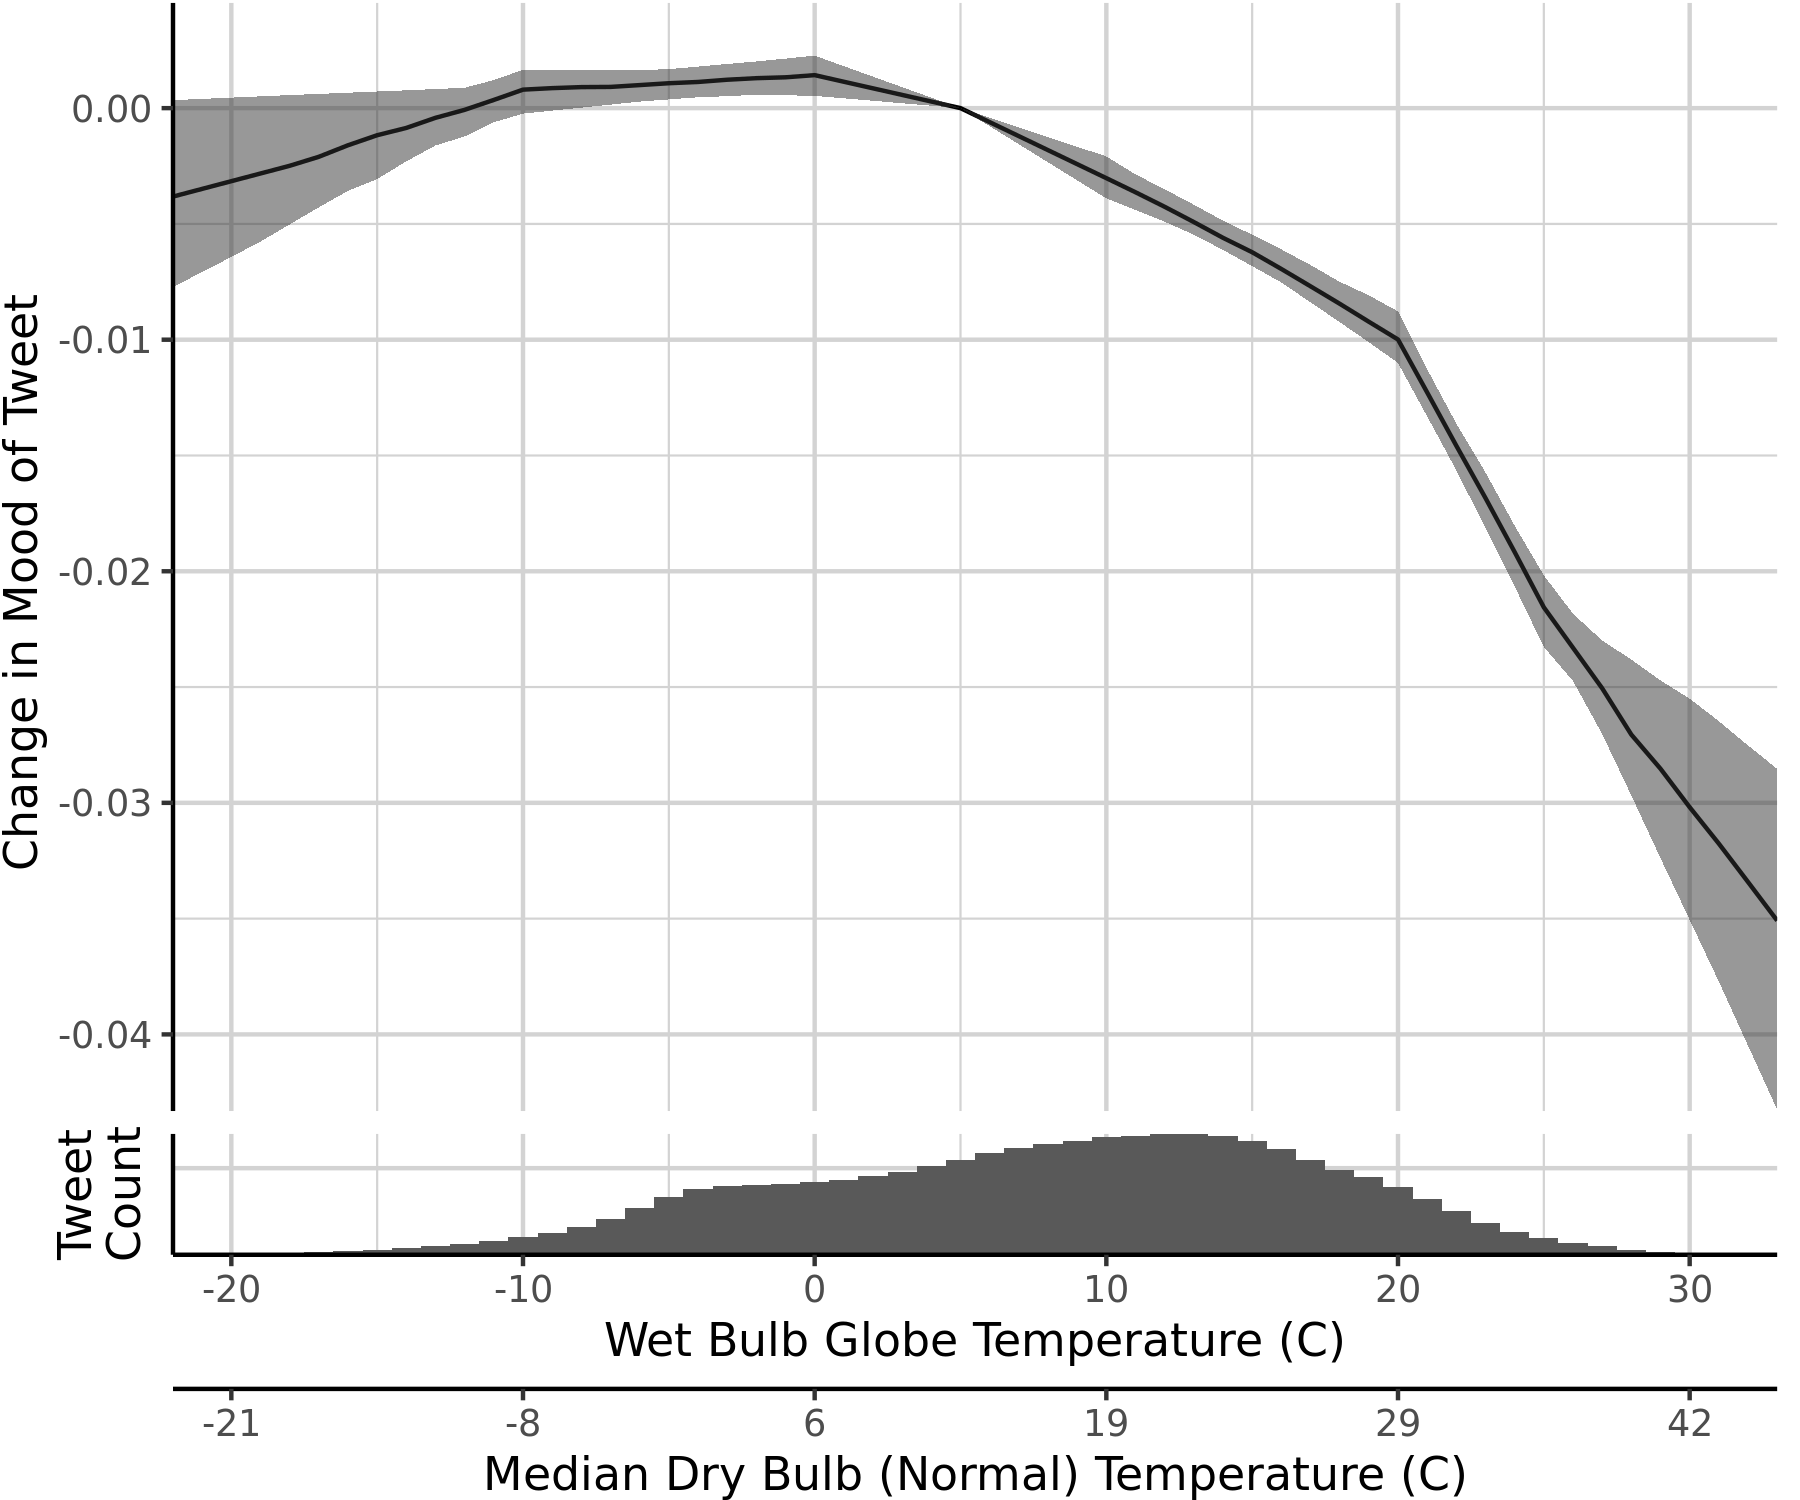
\includegraphics[width=0.6\linewidth]{../res/hedono-wbgt.png}
  \caption{Effects of temperature on mood, measured with the hedonometer method.}
\end{figure}

\begin{figure}[H]
  \centering
  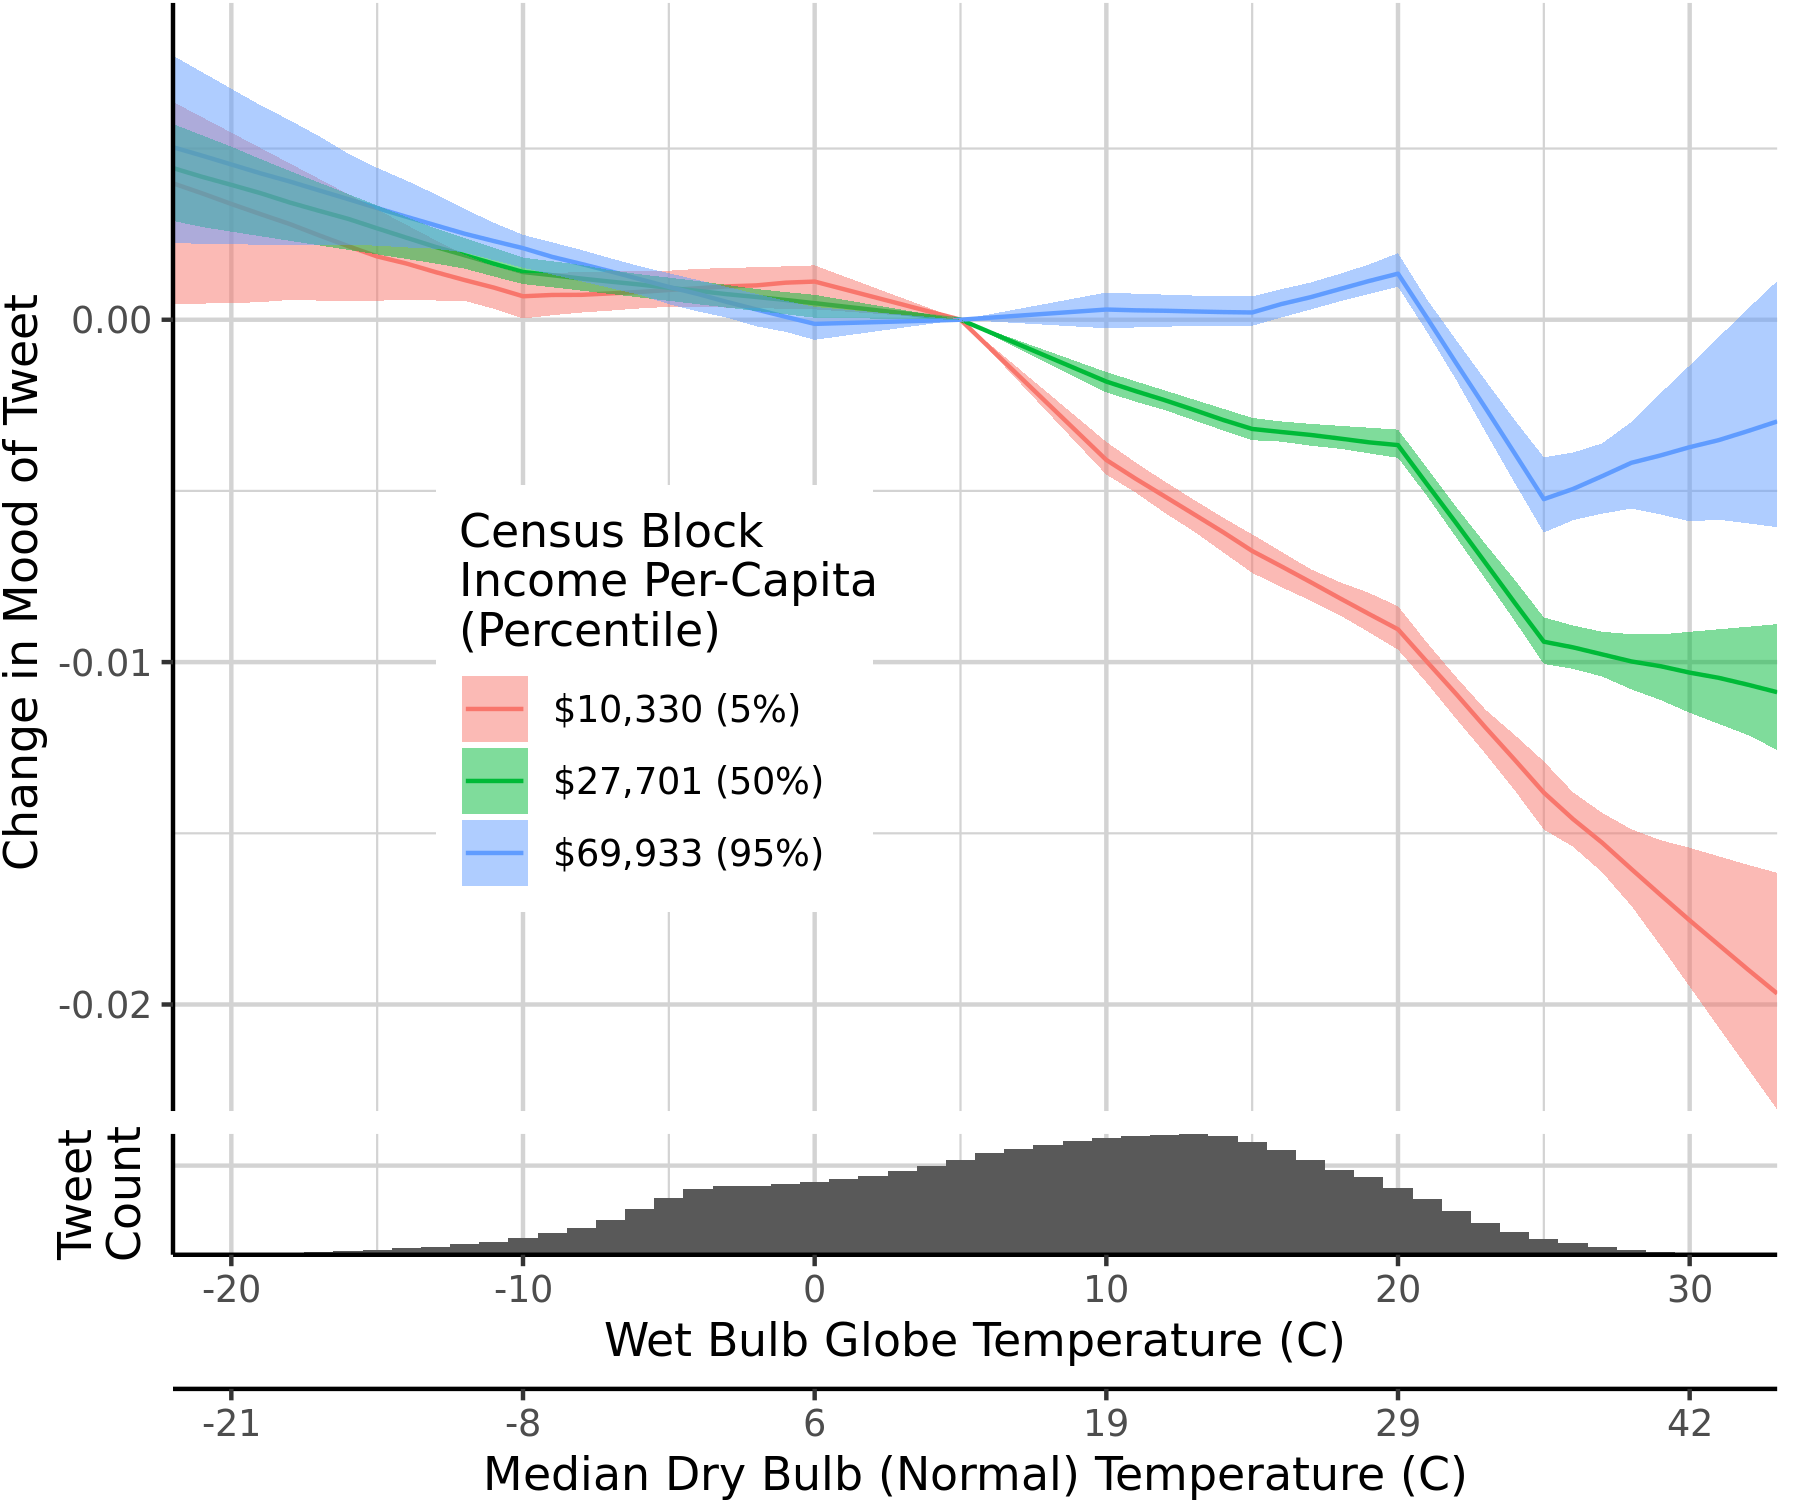
\includegraphics[width=0.6\linewidth]{../res/hedono-wbgt-income.png}
  \caption{Effects of temperature on mood and moderated by income, measured with the hedonometer method.}
\end{figure}

\begin{figure}[H]
  \centering
  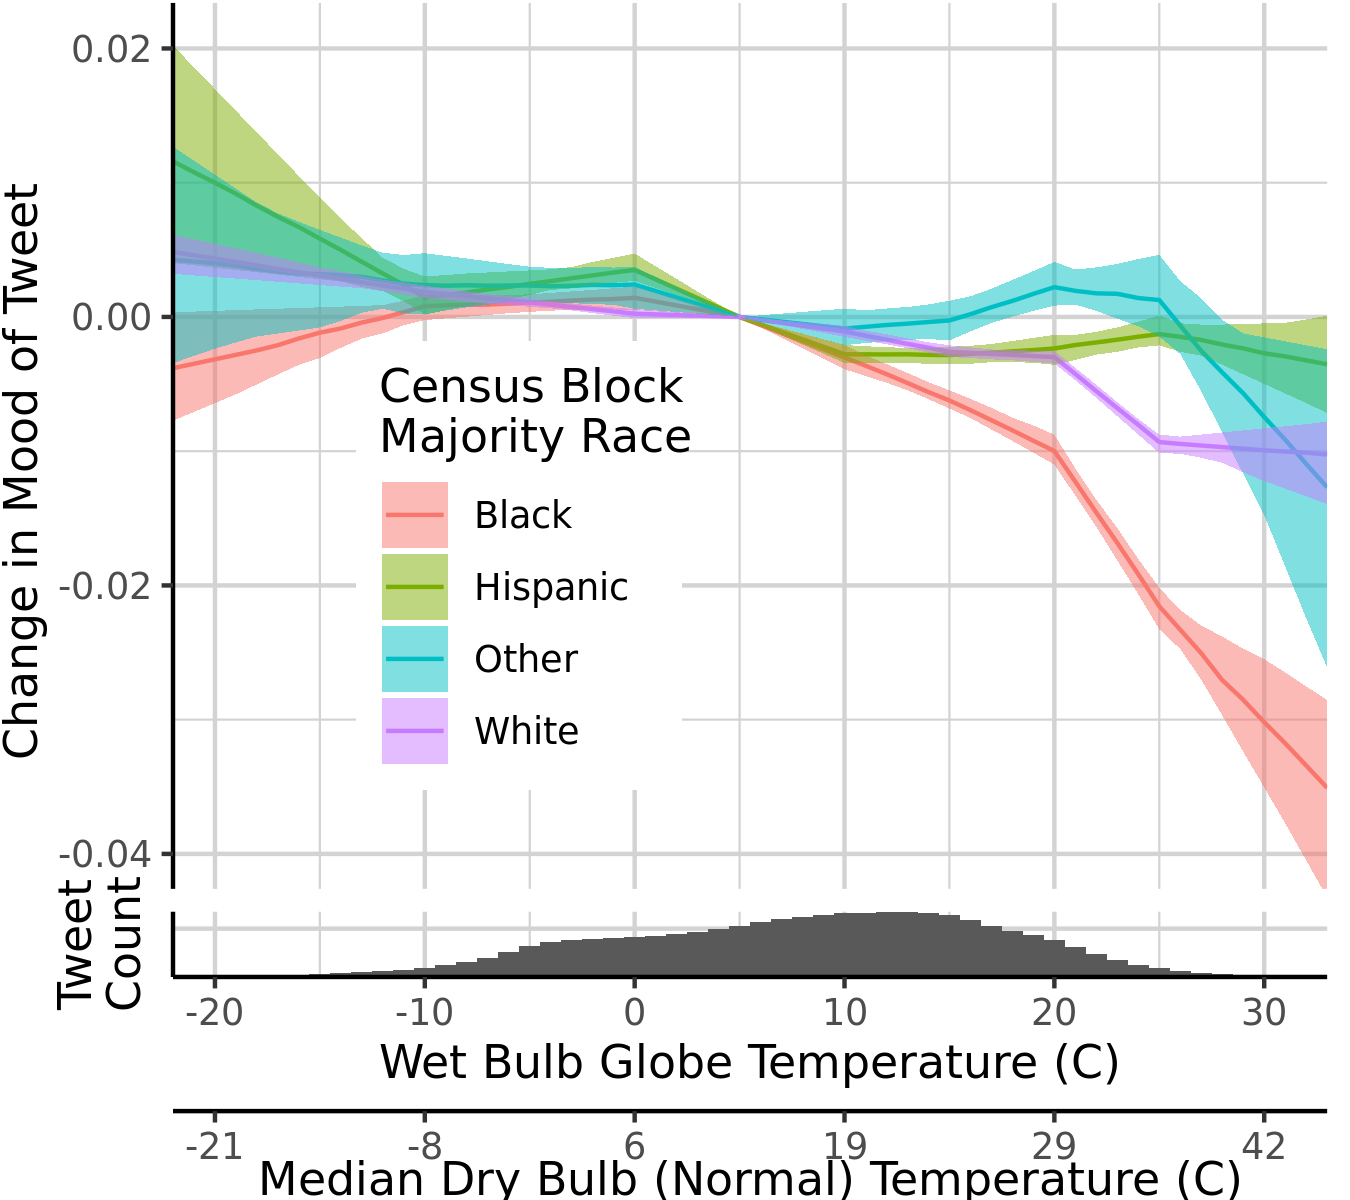
\includegraphics[width=0.6\linewidth]{../res/hedono-wbgt-race_q.png}
  \caption{Effects of temperature on mood and moderated by race, measured with the hedonometer method.}
\end{figure}

\subsection{AFINN}

AFINN is another wordlist used in mood analysis and designed for microblogs like twitter \cite{nielsen2011new}.

\begin{figure}[H]
  \centering
  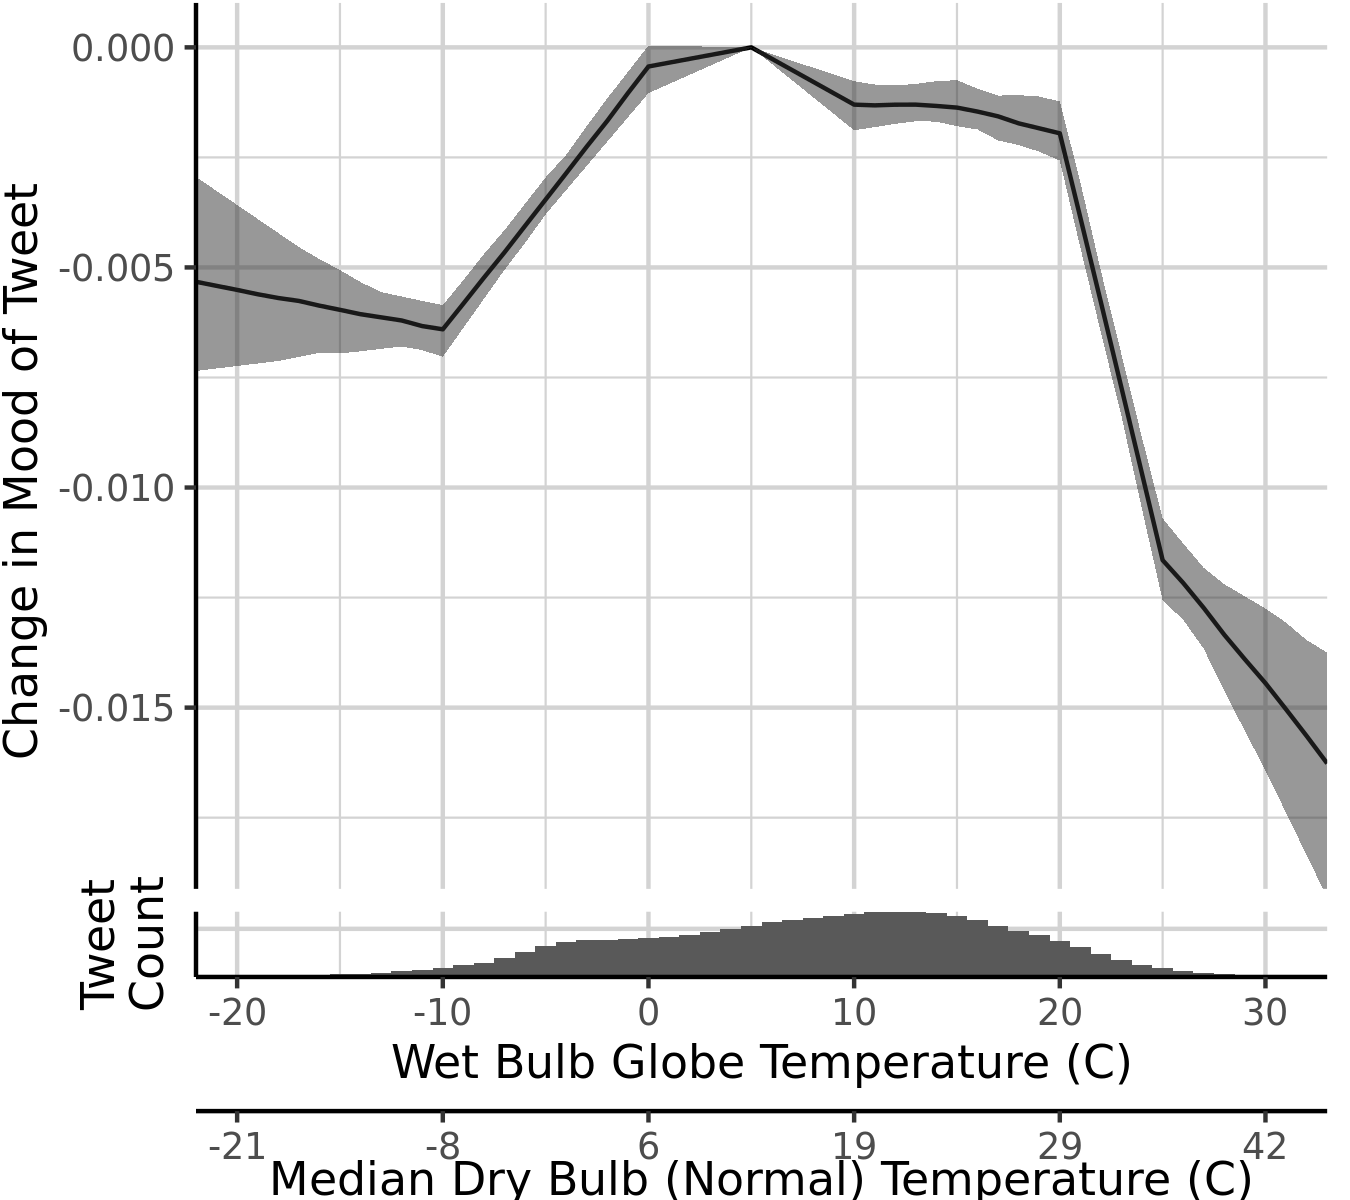
\includegraphics[width=0.6\linewidth]{../res/afinn-wbgt.png}
  \caption{Effects of temperature on mood, measured with the AFINN method.}
\end{figure}

\begin{figure}[H]
  \centering
  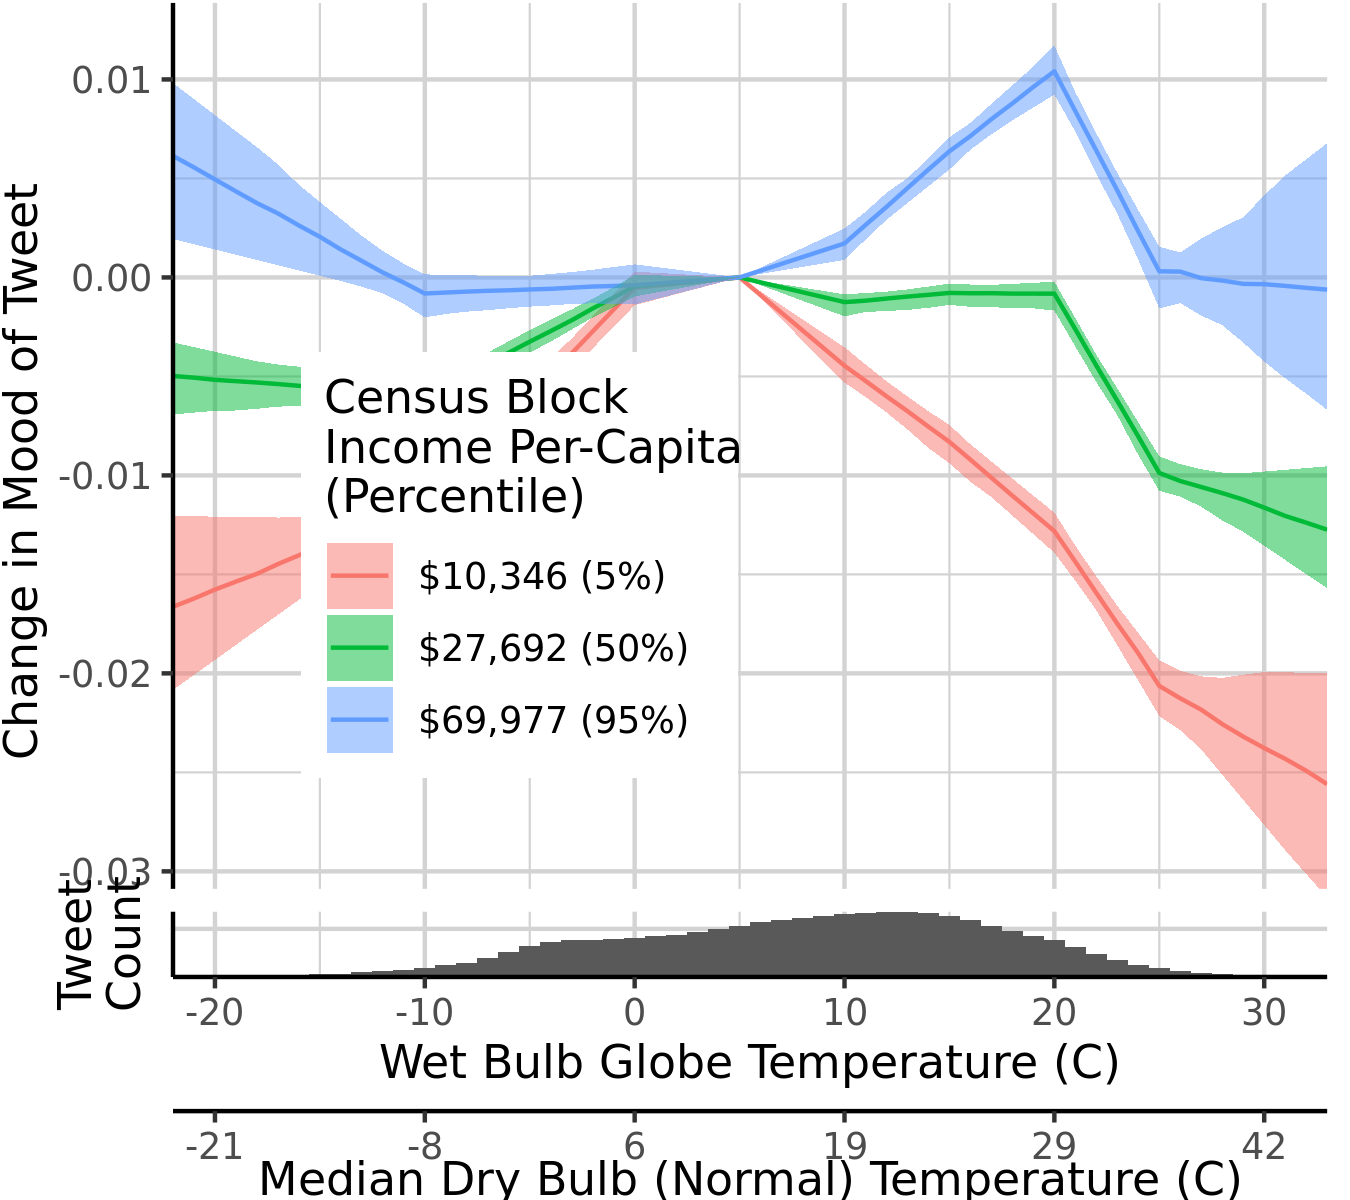
\includegraphics[width=0.6\linewidth]{../res/afinn-wbgt-income.png}
  \caption{Effects of temperature on mood and moderated by income, measured with the AFINN method.}
\end{figure}

\begin{figure}[H]
  \centering
  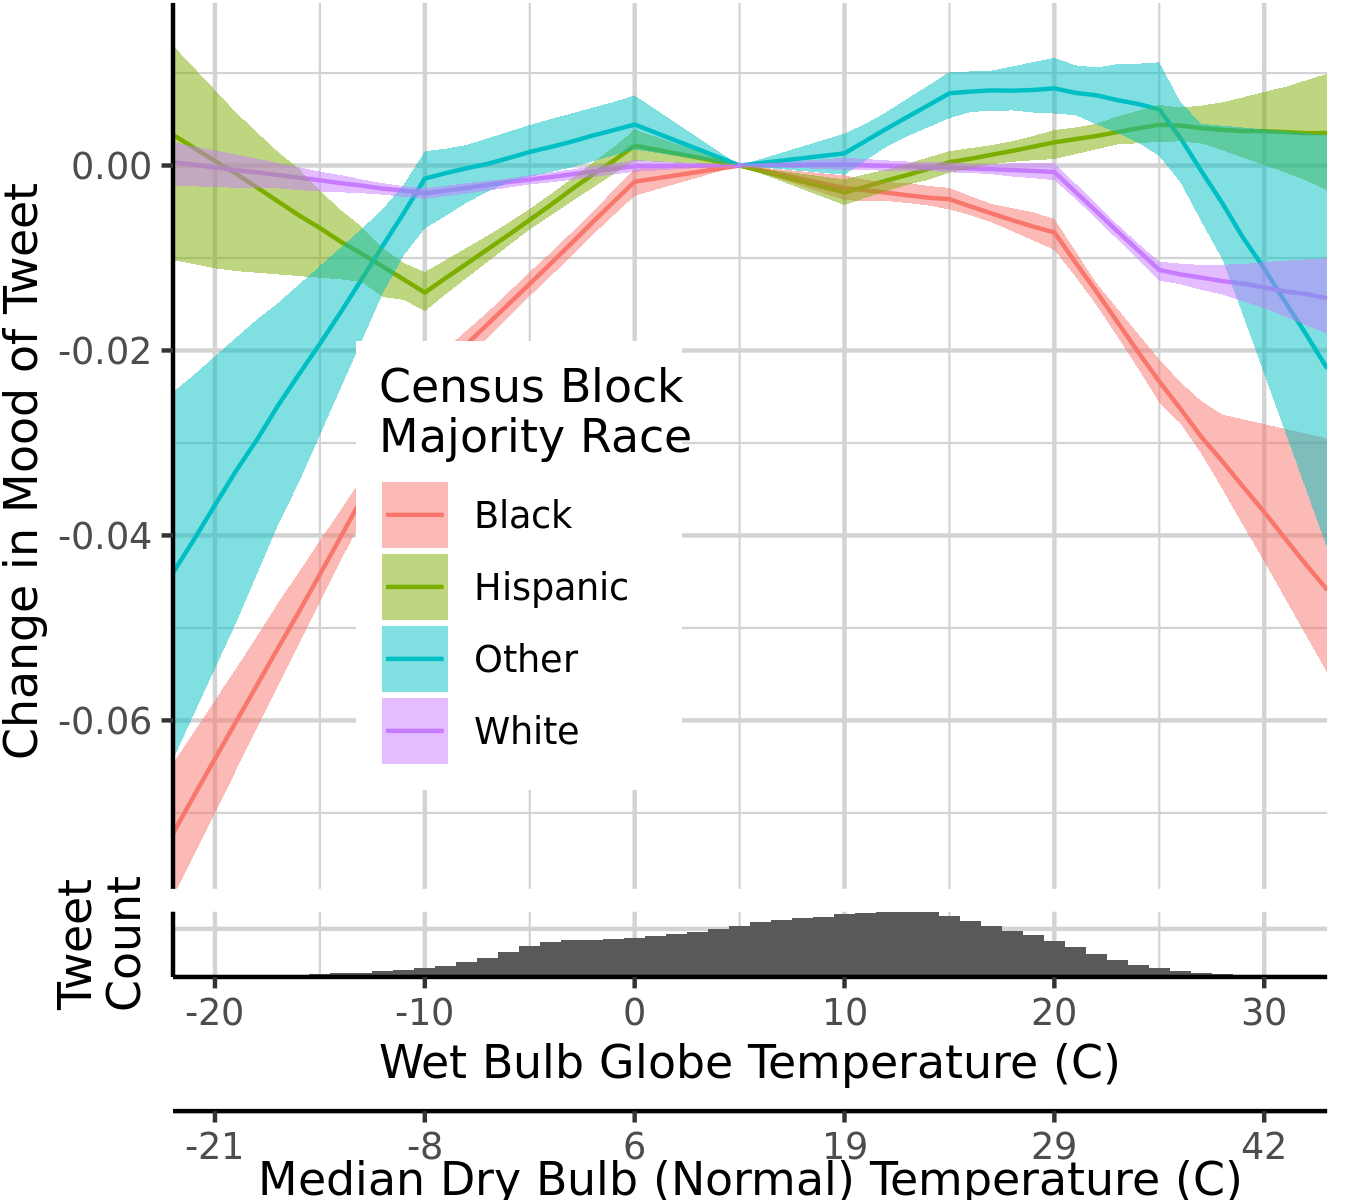
\includegraphics[width=0.6\linewidth]{../res/afinn-wbgt-race_q.png}
  \caption{Effects of temperature on mood and moderated by race, measured with the AFINN method.}
\end{figure}

\newpage
\section{Alternative Interaction Variables}
For our main analysis, we treated income as a continuous (log-transformed) variable and race as a categorical variable.  We ran similar analyses with income as a categorical variable and race as a continuous variable (the percent of a census block's population that was non-white/minority).

\begin{figure}[H]
  \centering
  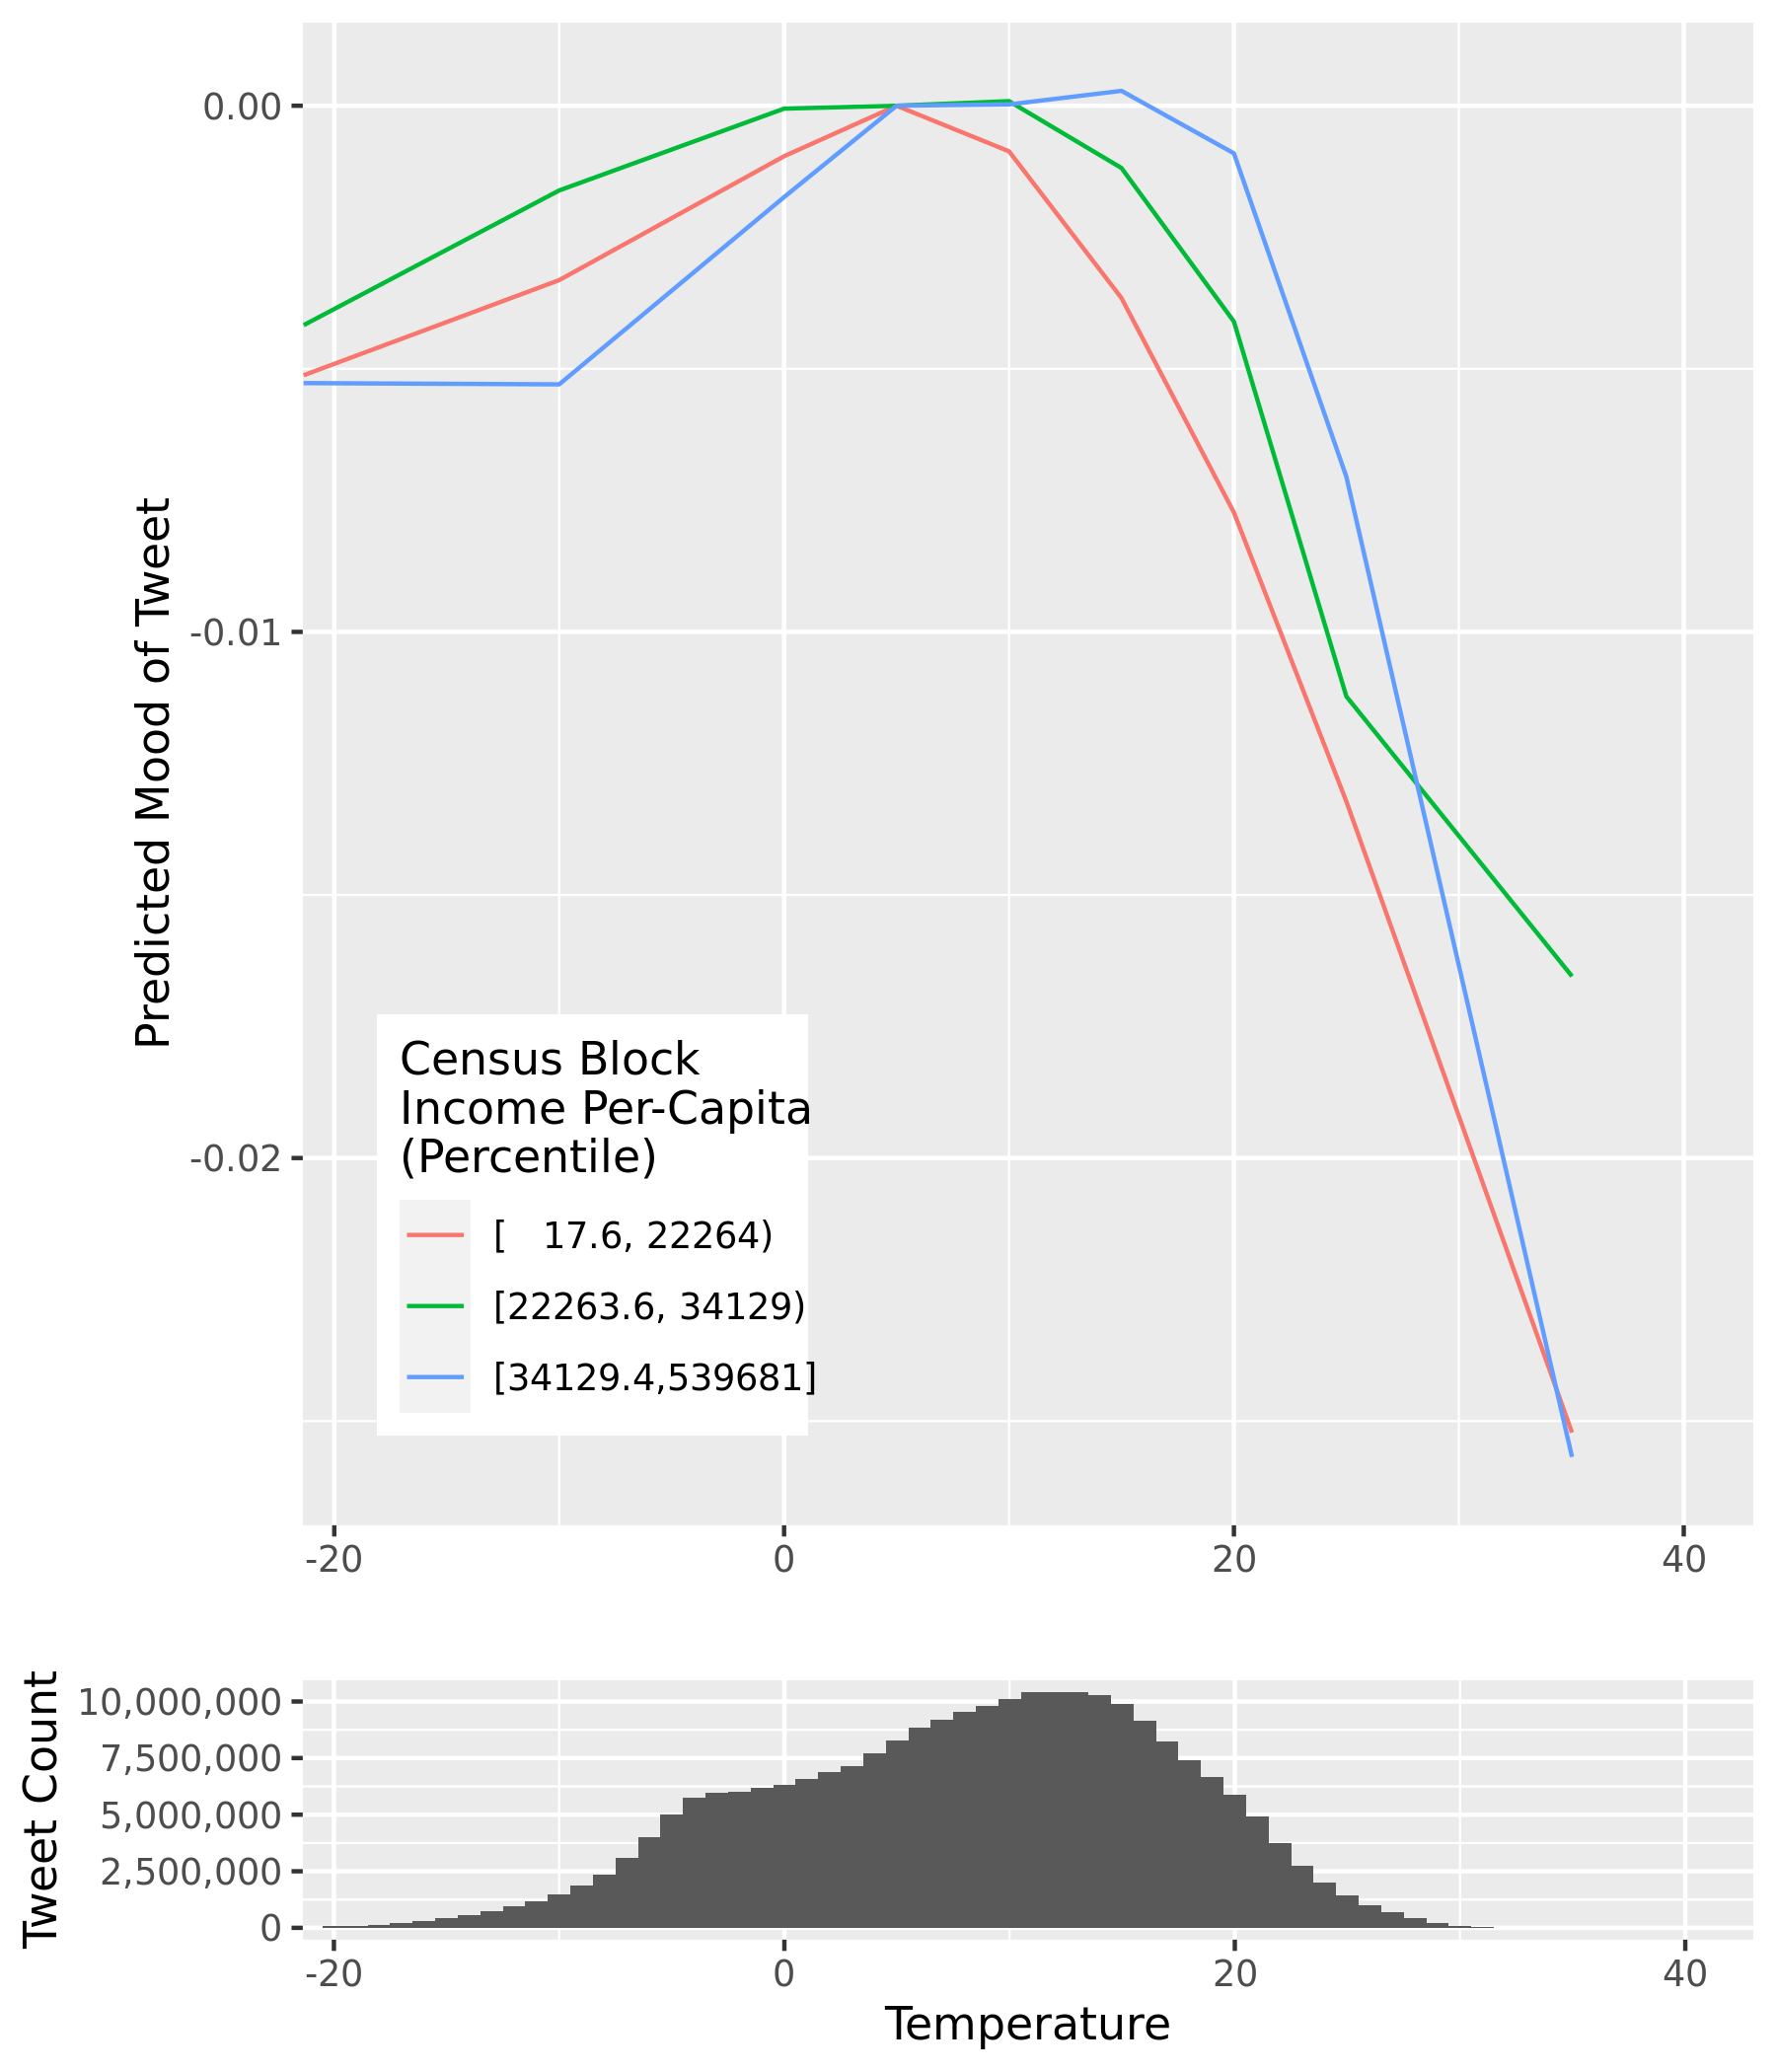
\includegraphics[width=0.6\linewidth]{../res/wbgt-income_q.png}
  \caption{Effect of temperature on mood and moderated by income, with income as a categorical variable.}
\end{figure}

\begin{figure}[H]
  \centering
  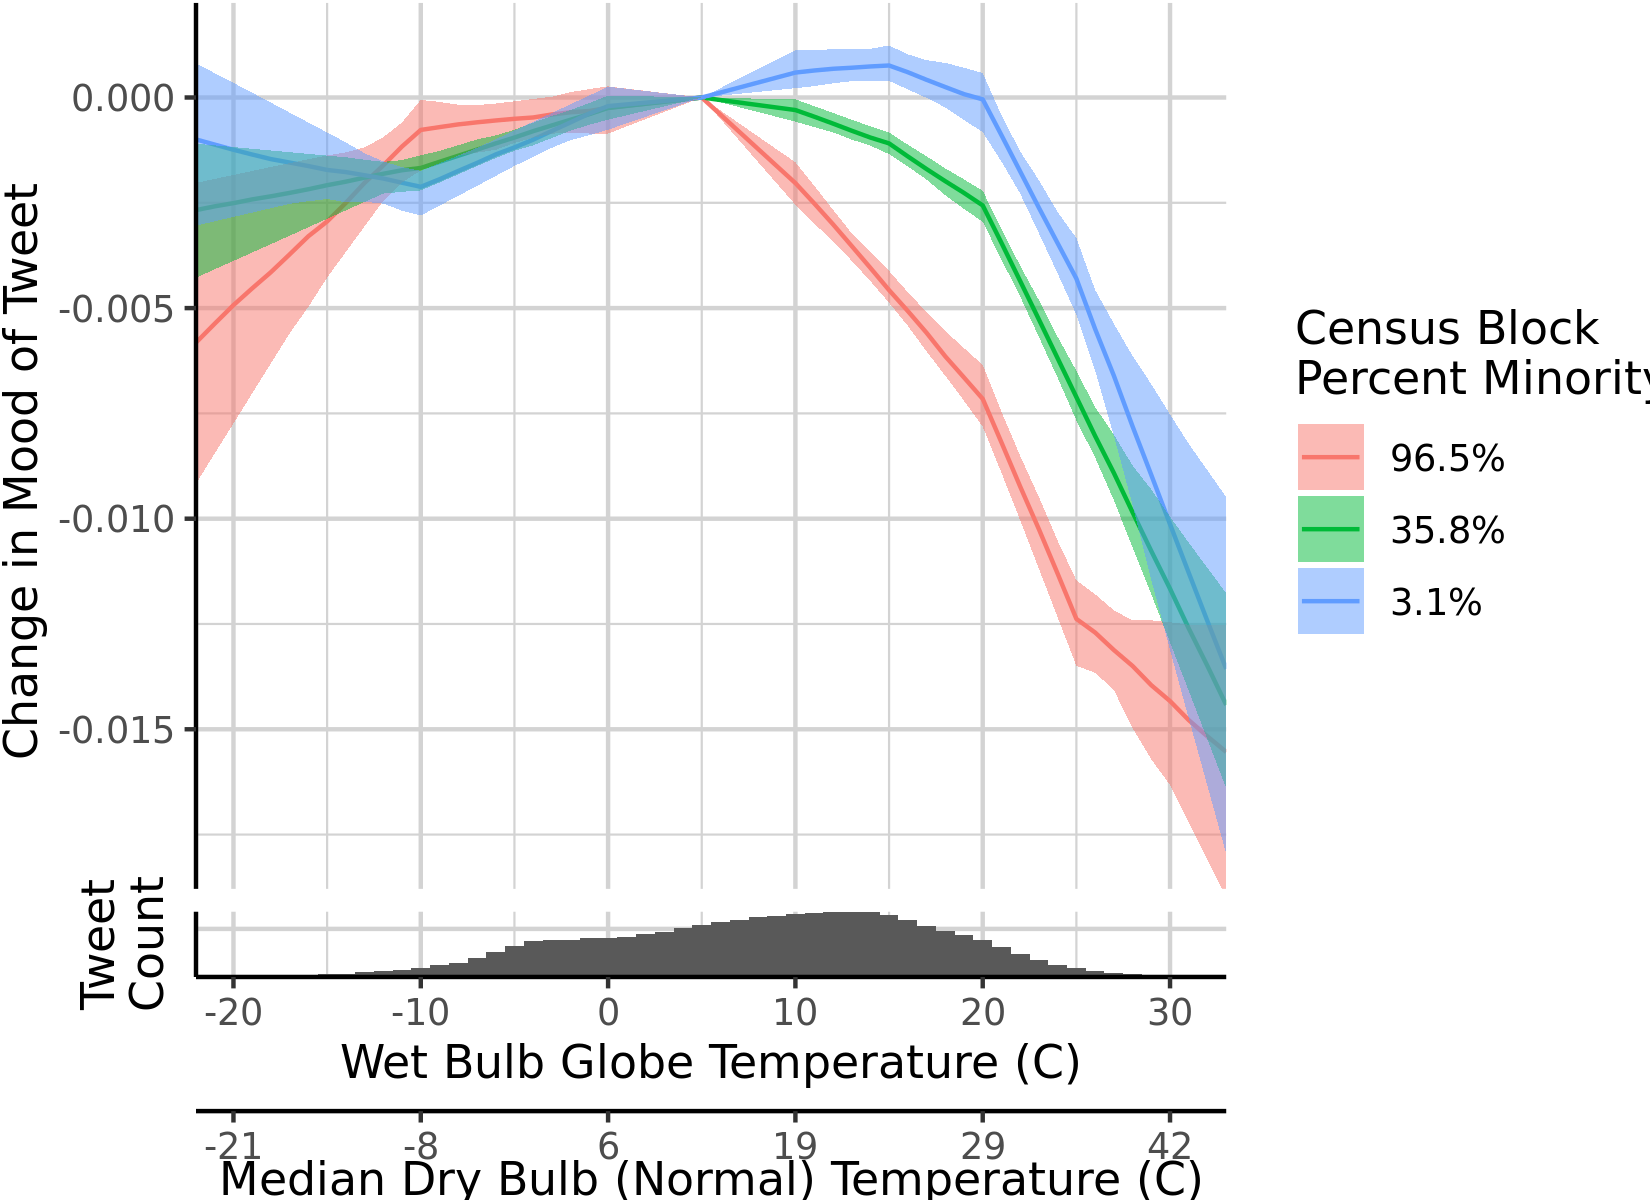
\includegraphics[width=0.6\linewidth]{../res/wbgt-race.png}
  \caption{Effect of temperature on mood and moderated by race, with race as a continuous variable.}
\end{figure}

\newpage
\section{Effects of Precipitation and Sunshine}
While our main variable of interest was temperature as measured by Wet Bulb Globe Temperature, we also interacted our variables of interest with a binary variable for whether it was raining or not, as well as a continuous variable for the amount of shortwave radiation in ($W/m^2$), or sunshine.

\begin{figure}[H]
  \centering
  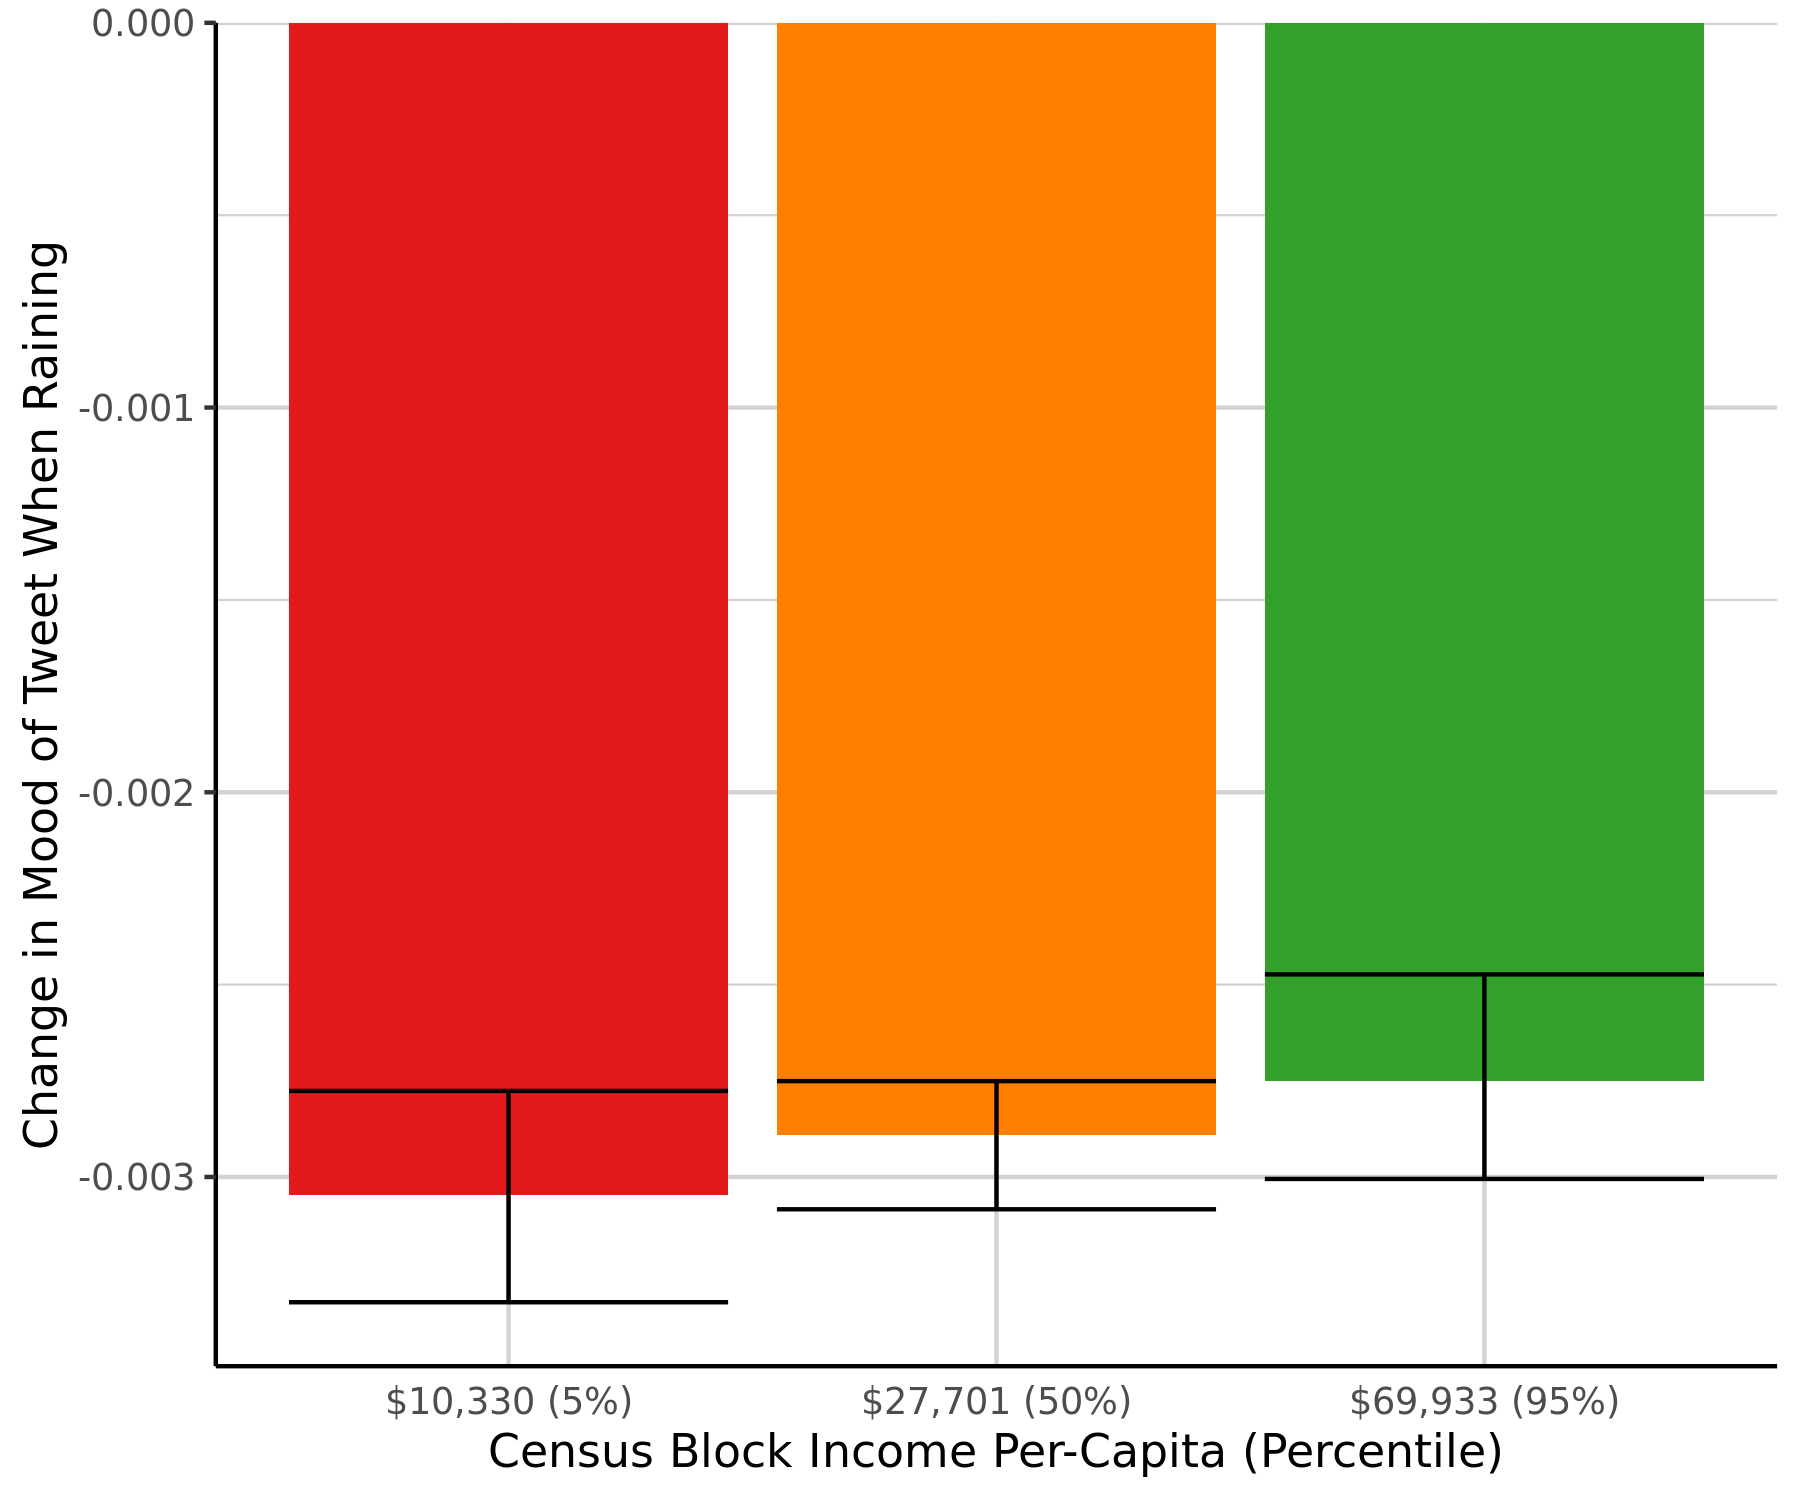
\includegraphics[width=0.6\linewidth]{../res/raining-income.png}
  \caption{Effect of rain on mood and moderated by income.}
  \label{fig:timeseries}
\end{figure}

\begin{figure}[H]
  \centering
  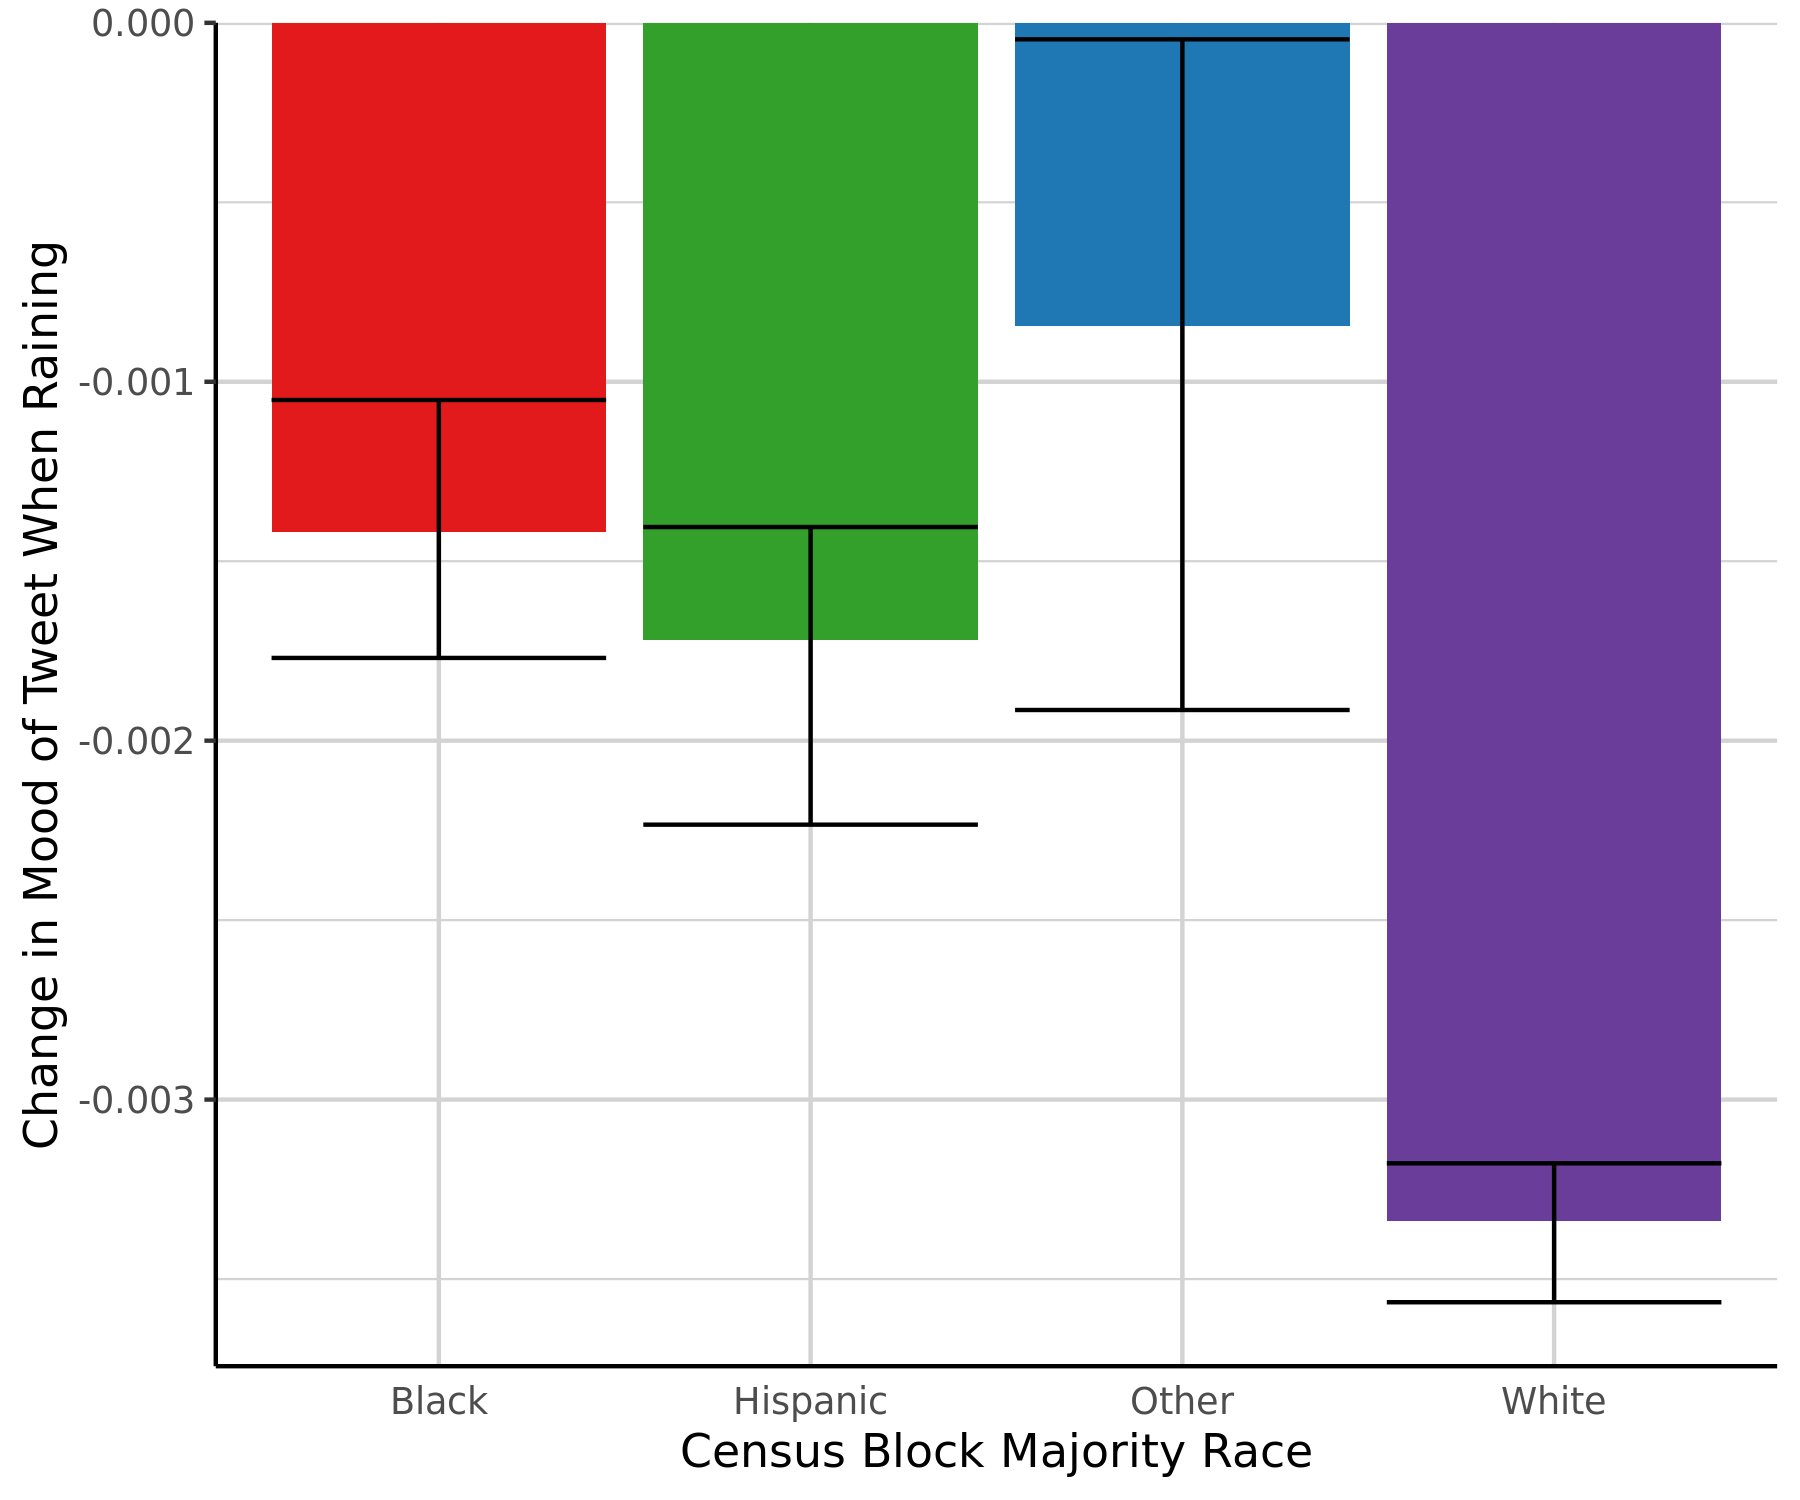
\includegraphics[width=0.6\linewidth]{../res/raining-race_q.png}
  \caption{Effect of rain on mood and moderated by race.}
  \label{fig:timeseries}
\end{figure}


\begin{figure}[H]
  \centering
  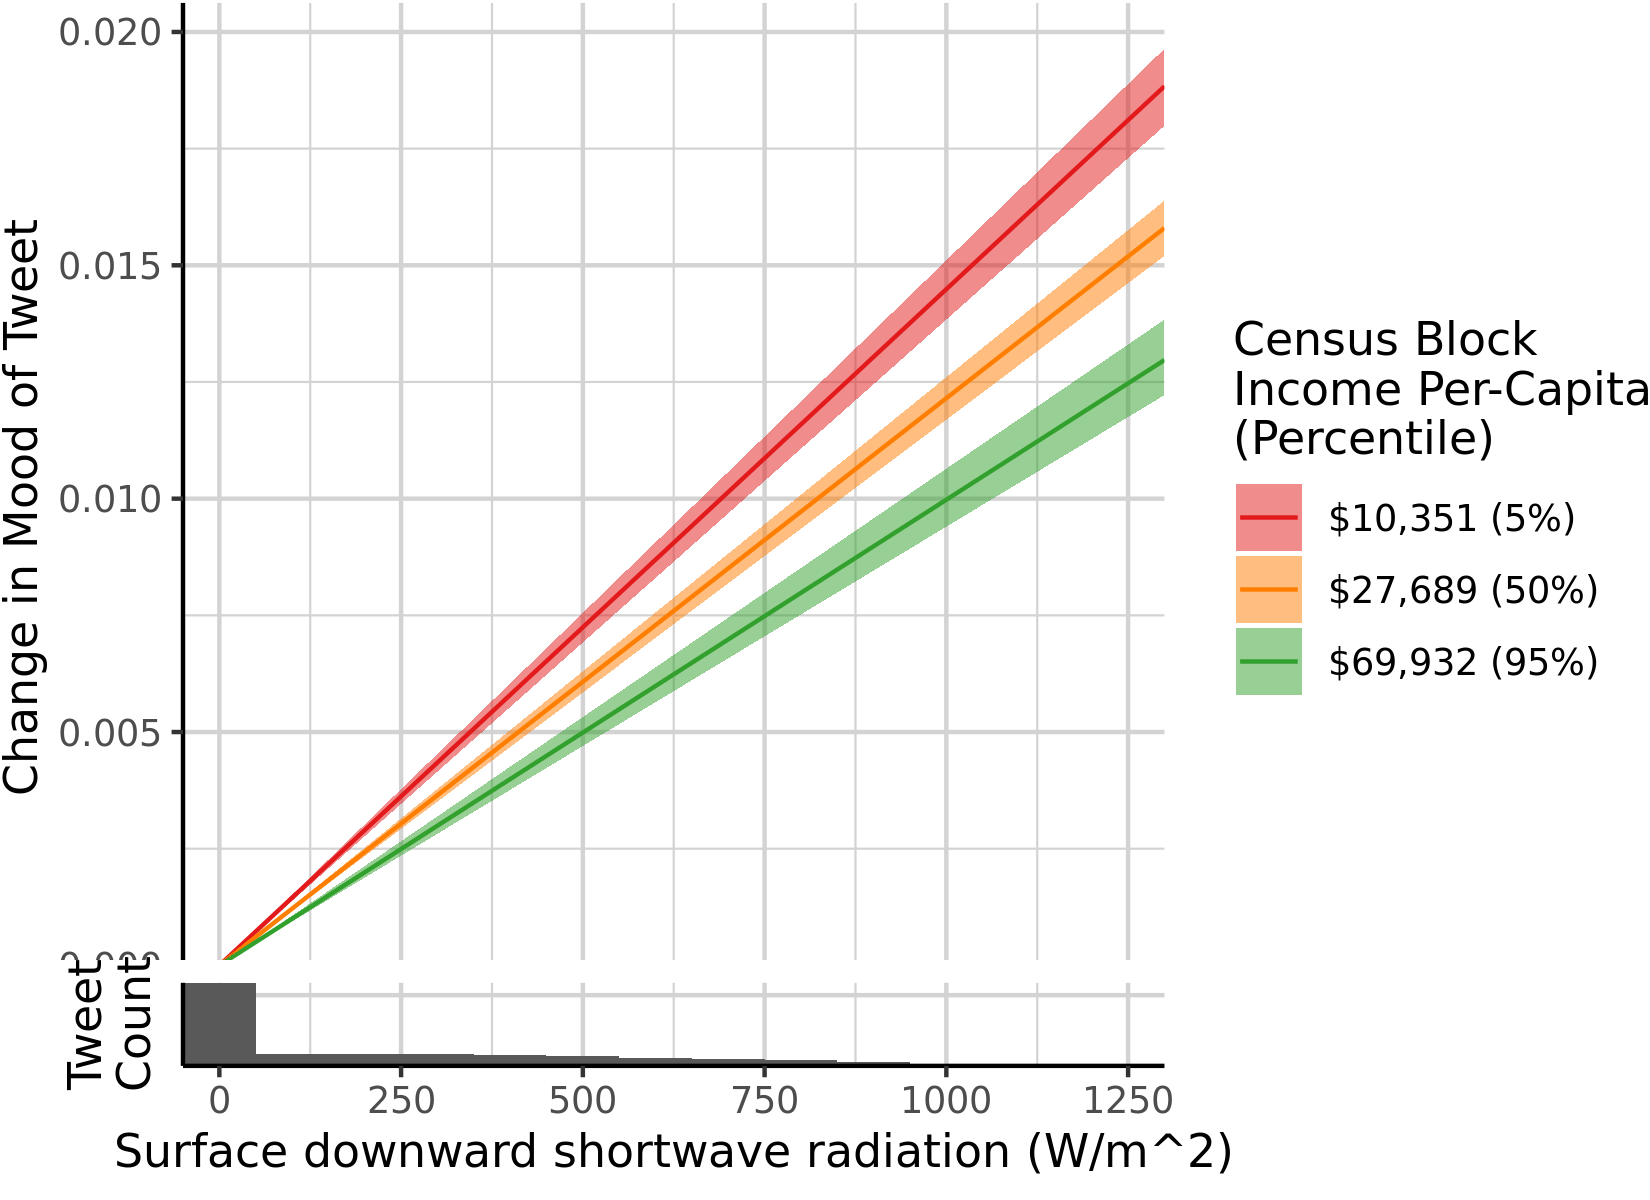
\includegraphics[width=0.6\linewidth]{../res/srad-income.png}
  \caption{Effect of sunshine on mood and moderated by income.}
  \label{fig:timeseries}
\end{figure}

\begin{figure}[H]
  \centering
  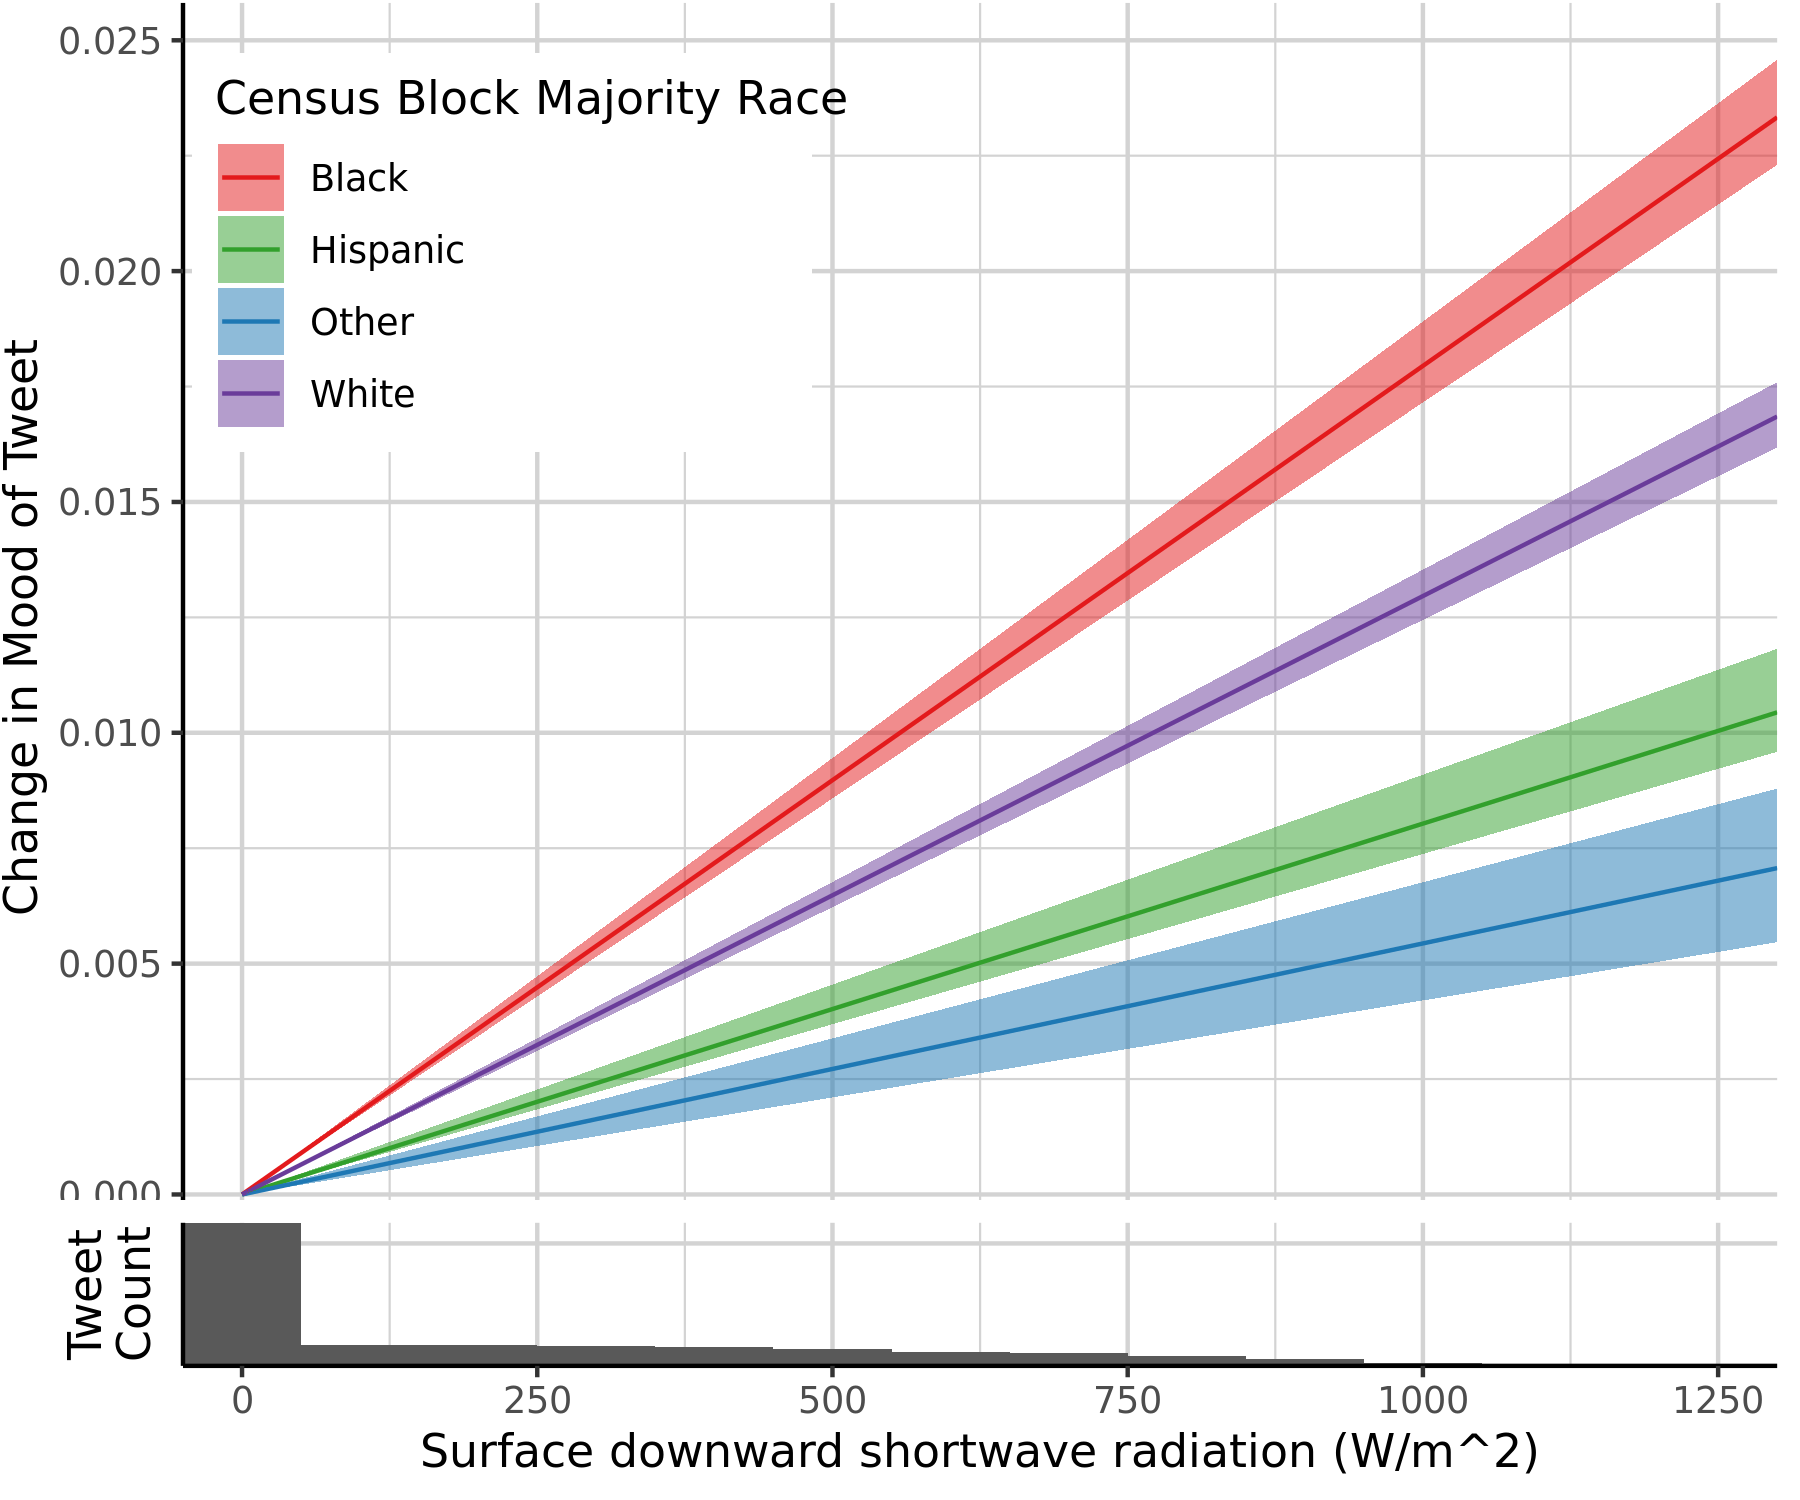
\includegraphics[width=0.6\linewidth]{../res/srad-race_q.png}
  \caption{Effect of sunshine on mood and moderated by race.}
  \label{fig:timeseries}
\end{figure}

\newpage
\section*{Temperature Effects by Combined Statistical Area}
To explore whether cultural or environmental baselines may affect the relationship between heat and mood, we examine the impact of temperature on mood across Combined Statistical Areas (CSAs) and Metropolitan Statistical Areas (MSAs) containing over 1 million people (hereafter: city regions). We find that higher temperatures are associated with declining mood in 83.6\% of city regions (see Fig. \ref{fig:map}) and the effect is significant in 35.3\% of these. Furthermore, we find no significant association between higher temperatures and increased mood in any of the cities.

For this analysis by city, we run models with a similar form to Model 2, including the same fixed effects, although we fit a linear effect for $f_t()$.  Because we are not accounting for non-linearities in $f_t()$, we exclude tweets with a WBGT of less than 5\textdegree C, as our initial analysis showed that this is the temperature at which mood peaks.

\begin{figure}[H]
\centering
  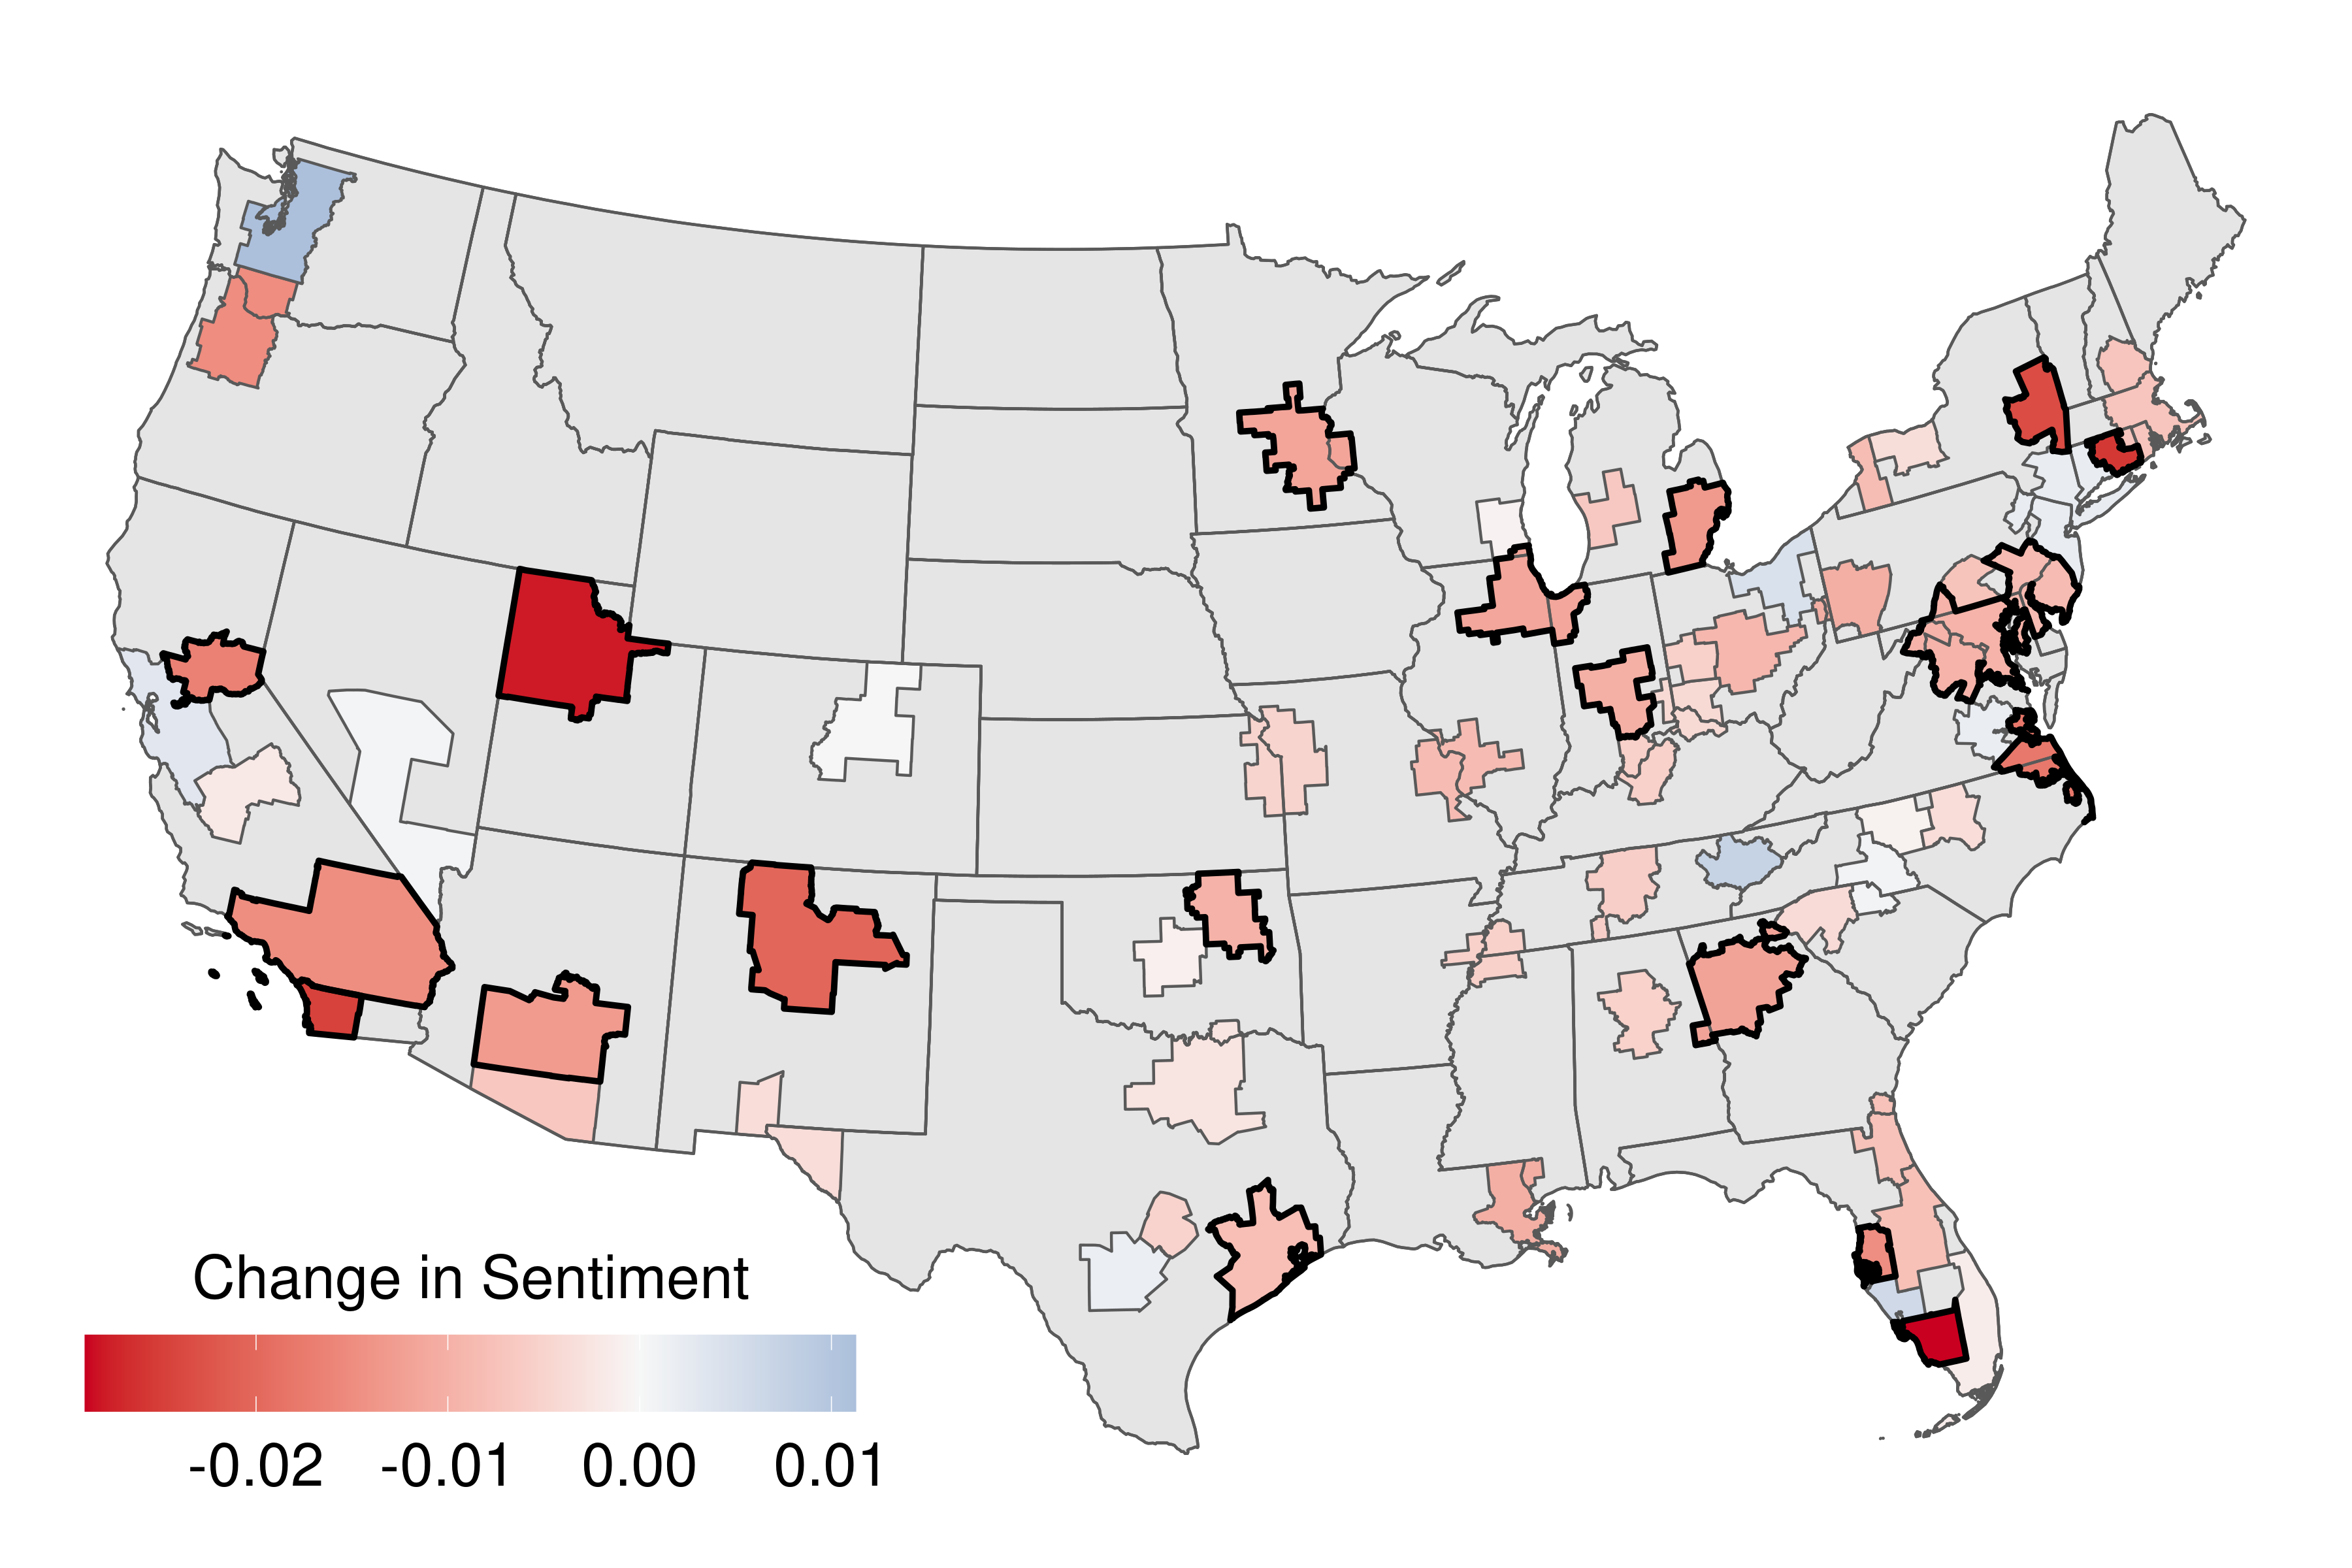
\includegraphics[width=\linewidth]{../res/map_wbgt.png}
    \caption{The change in mood for a 25-degree increase in WBGT for city regions with a population of over 1 million.  For cities shown with a dark outline, the effect is significant at a 95\% confidence interval.}
  \label{fig:map}
\end{figure}

\newpage
\section*{Interaction between Race and Income}
Given that both low-income and majority black neighborhoods are more vulnerable to heat waves, we model the combined effects of race and income together to explore the intersection of these two types of vulnerability. Specifically, we model how the relationship between temperature and mood is moderated by the interaction between a neighborhood's per-capita income and the percentage of a neighborhood's inhabitants that are black. Additionally, we compare AICs for models with no term for vulnerability, a race term for vulnerability, an income term for vulnerability, and both race and income terms for vulnerability.

\begin{minipage}{.65\textwidth}
\centering
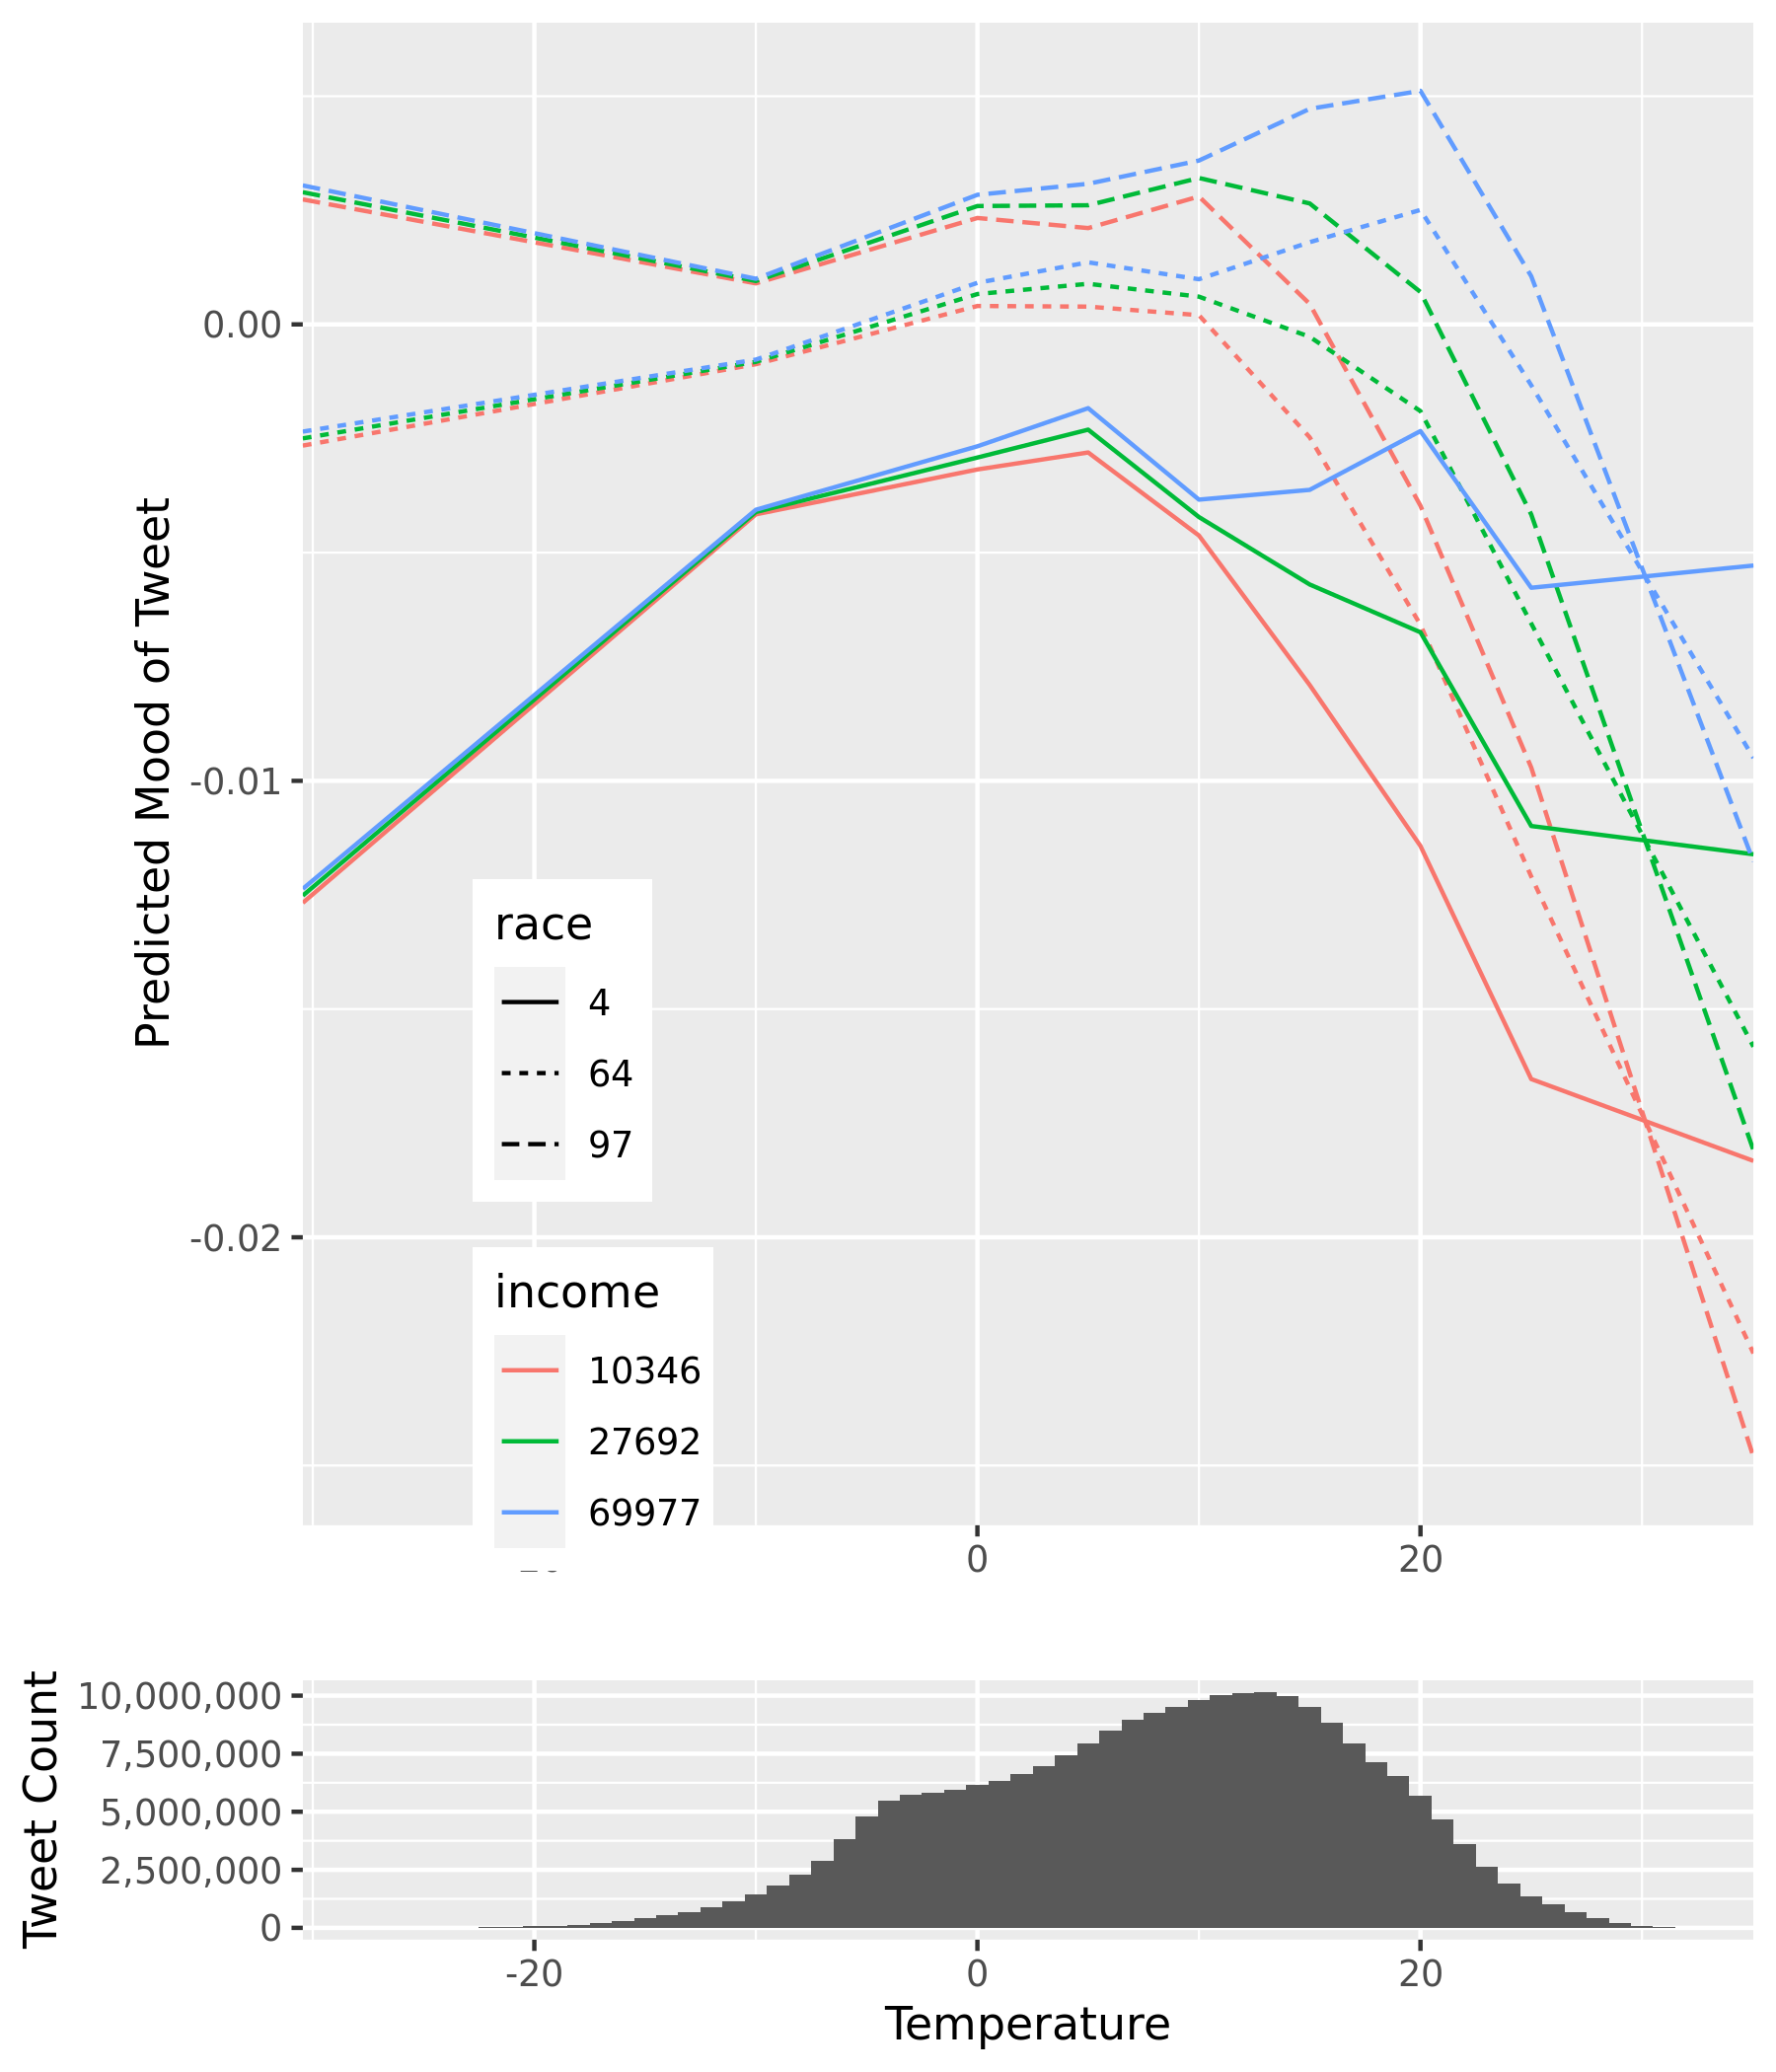
\includegraphics[width=\textwidth]{../res/wbgt-income-race.png}
\captionof{figure}{Relationship between WBGT and mood from text in tweets, moderated by the interaction of race and income.}
\label{fig:race-income}
\end{minipage}\hfill
\begin{minipage}{.35\textwidth}
\centering
\begin{tabular}{| l | l |}
\hline
Terms & AIC \\
\hline
Neither & 277,270,561 \\
Income & 277,182,239 \\
Race & 277,143,579 \\
Both & 277,108,676 \\
\hline
\end{tabular}
\captionof{table}{Akaike information criterion (AIC) of models with interaction terms for race, income, both race and income, as well as neither race nor income. The model with the best fit by AIC includes both race and income interaction terms.}
\label{tab:aics}
\end{minipage}

Graphing the combined effects of race and income, we find that race has a larger impact on vulnerability than income (see Fig. \ref{fig:race-income}). A Black neighborhood at any income level will be much more impacted by heat than a poor neighborhood with few black inhabitants. Additionally, neighborhoods that are largely black are also more affected by cold temperatures, although there is no clear effect of income moderating the relationship between cold temperatures and mood. Using AIC as an indicator of how different terms affect model quality (see Tab. \ref{tab:aics}), we find that a model including both terms performs the best, indicating that both race and income matter for the impact of heat on mood. However, including only a race term improves the model more than including only an income term, further supporting the conclusion that race is more important than income for explaining the vulnerability of mood to heat.



\newpage
\section{Weather Terms}
For all of our analysis, we excluded tweets that contained the following weather-related terms: aerovane, air, airstream, altocumulus, altostratus, anemometer, anemometers, anticyclone, anticyclones, arctic, arid, aridity, atmosphere, atmospheric, autumn, autumnal, balmy, baroclinic, barometer, barometers, barometric, blizzard, blizzards, blustering, blustery, blustery, breeze, breezes, breezy, brisk, calm, celsius, chill, chilled, chillier, chilliest, chilly, chinook, cirrocumulus, cirrostratus, cirrus, climate, climates, cloud, cloudburst, cloudbursts, cloudier, cloudiest, clouds, cloudy, cold, colder, coldest, condensation, contrail, contrails, cool, cooled, cooling, cools, cumulonimbus, cumulus, cyclone, cyclones, damp, damp, damper, damper, dampest, dampest, degree, degrees, deluge, dew, dews, dewy, doppler, downburst, downbursts, downdraft, downdrafts, downpour, downpours, dried, drier, dries, driest, drizzle, drizzled, drizzles, drizzly, drought, droughts, dry, dryline, fall, farenheit, flood, flooded, flooding, floods, flurries, flurry, fog, fogbow, fogbows, fogged, fogging, foggy, fogs, forecast, forecasted, forecasting, forecasts, freeze, freezes, freezing, frigid, frost, frostier, frostiest, frosts, frosty, froze, frozen, gale, gales, galoshes, gust, gusting, gusts, gusty, haboob, haboobs, hail, hailed, hailing, hails, haze, hazes, hazy, heat, heated, heating, heats, hoarfrost, hot, hotter, hottest, humid, humidity, hurricane, hurricanes, ice, iced, ices, icing, icy, inclement, landspout, landspouts, lightning, lightnings, macroburst, macrobursts, maelstrom, mercury, meteorologic, meteorologist, meteorologists, meteorology, microburst, microbursts, microclimate, microclimates, millibar, millibars, mist, misted, mists, misty, moist, moisture, monsoon, monsoons, mugginess, muggy, nexrad, nippy, NOAA, nor'easter, nor'easters, noreaster, noreasters, overcast, ozone, parched, parching, pollen, precipitate, precipitated, precipitates, precipitating, precipitation, psychrometer, radar, rain, rainboots, rainbow, rainbows, raincoat, raincoats, rained, rainfall, rainier, rainiest, raining, rains, rainy, sandstorm, sandstorms, scorcher, scorching, searing, shower, showering, showers, skiff, sleet, slicker, slickers, slush, slushy, smog, smoggier, smoggiest, smoggy, snow, snowed, snowier, snowiest, snowing, snowmageddon, snowpocalypse, snows, snowy, spring, sprinkle, sprinkles, sprinkling, squall, squalls, squally, storm, stormed, stormier, stormiest, storming, storms, stormy, stratocumulus, stratus, subtropical, summer, summery, sun, sunnier, sunniest, sunny, temperate, temperature, tempest, thaw, thawed, thawing, thaws, thermometer, thunder, thundered, thundering, thunders, thunderstorm, thunderstorms, tornadic, tornado, tornadoes, tropical, troposphere, tsunami, turbulent, twister, twisters, typhoon, typhoons, umbrella, umbrellas, vane, warm, warmed, warming, warms, warmth, waterspout, waterspouts, weather, wet, wetter, wettest, wind, windchill, windchills, windier, windiest, windspeed, windy, winter, wintery, and wintry.


\printbibliography

\end{document}
